%%%%%%%%%%%%%%%%%%%%%%%%%%%%%%%%%%%%%%%%%%%%%%%%%%%%%%%%%%%%%%%%%%%%%%%%%%%%
%%%%%                          ANNEXE 1                               %%%%%%
%%%%%%%%%%%%%%%%%%%%%%%%%%%%%%%%%%%%%%%%%%%%%%%%%%%%%%%%%%%%%%%%%%%%%%%%%%%%

\appendix
\renewcommand\chaptername{Appendix~}
\phantomsection 

\lhead[\fancyplain{}{\leftmark}]%Pour les pages paires \bfseries
      {\fancyplain{}{}} %Pour les pages impaires
\chead[\fancyplain{}{}]%
      {\fancyplain{}{}}
\rhead[\fancyplain{}{}]%Pour les pages paires 
      {\fancyplain{}{\rightmark}}%Pour les pages impaires \bfseries
\lfoot[\fancyplain{}{}]%
      {\fancyplain{}{}}
\cfoot[\fancyplain{}{\thepage}]%\bfseries
      {\fancyplain{}{\thepage}} %\bfseries
\rfoot[\fancyplain{}{}]%
     {\fancyplain{}{\scriptsize}}


%%%%%%%%%%%%%%%%%%%%%%%%%%%%%%%%%%%%%%%%%%%%%%%%%%%%%%%%%%%%%%%%%%%%%%%%%%
%%%%%                      Start part here                          %%%%%%
%%%%%%%%%%%%%%%%%%%%%%%%%%%%%%%%%%%%%%%%%%%%%%%%%%%%%%%%%%%%%%%%%%%%%%%%%%

\chapter{Appendix A on Robustness assessment}
\label{Ann:1}

%==============================================================================	Résumé du chapitre

\begin{center}
\rule{0.7\linewidth}{.5pt}
\begin{minipage}{0.7\linewidth}
\smallskip

\textit{
Supplementary figures for Chapter 4 on \nameref{ch:4}, for the running and cycling tasks. \newline\newline All details on methods and results are provided in the forementioned chapter.
}

%\smallskip
\end{minipage}
\smallskip
\rule{0.7\linewidth}{.5pt}
\end{center}

%\adjustmtc
\minitoc
\newpage

\section{Robustness: Running task results}

\begin{figure}[!ht]
	\centering
	\def\svgwidth{1\columnwidth}
	\fontsize{10pt}{10pt}\selectfont
	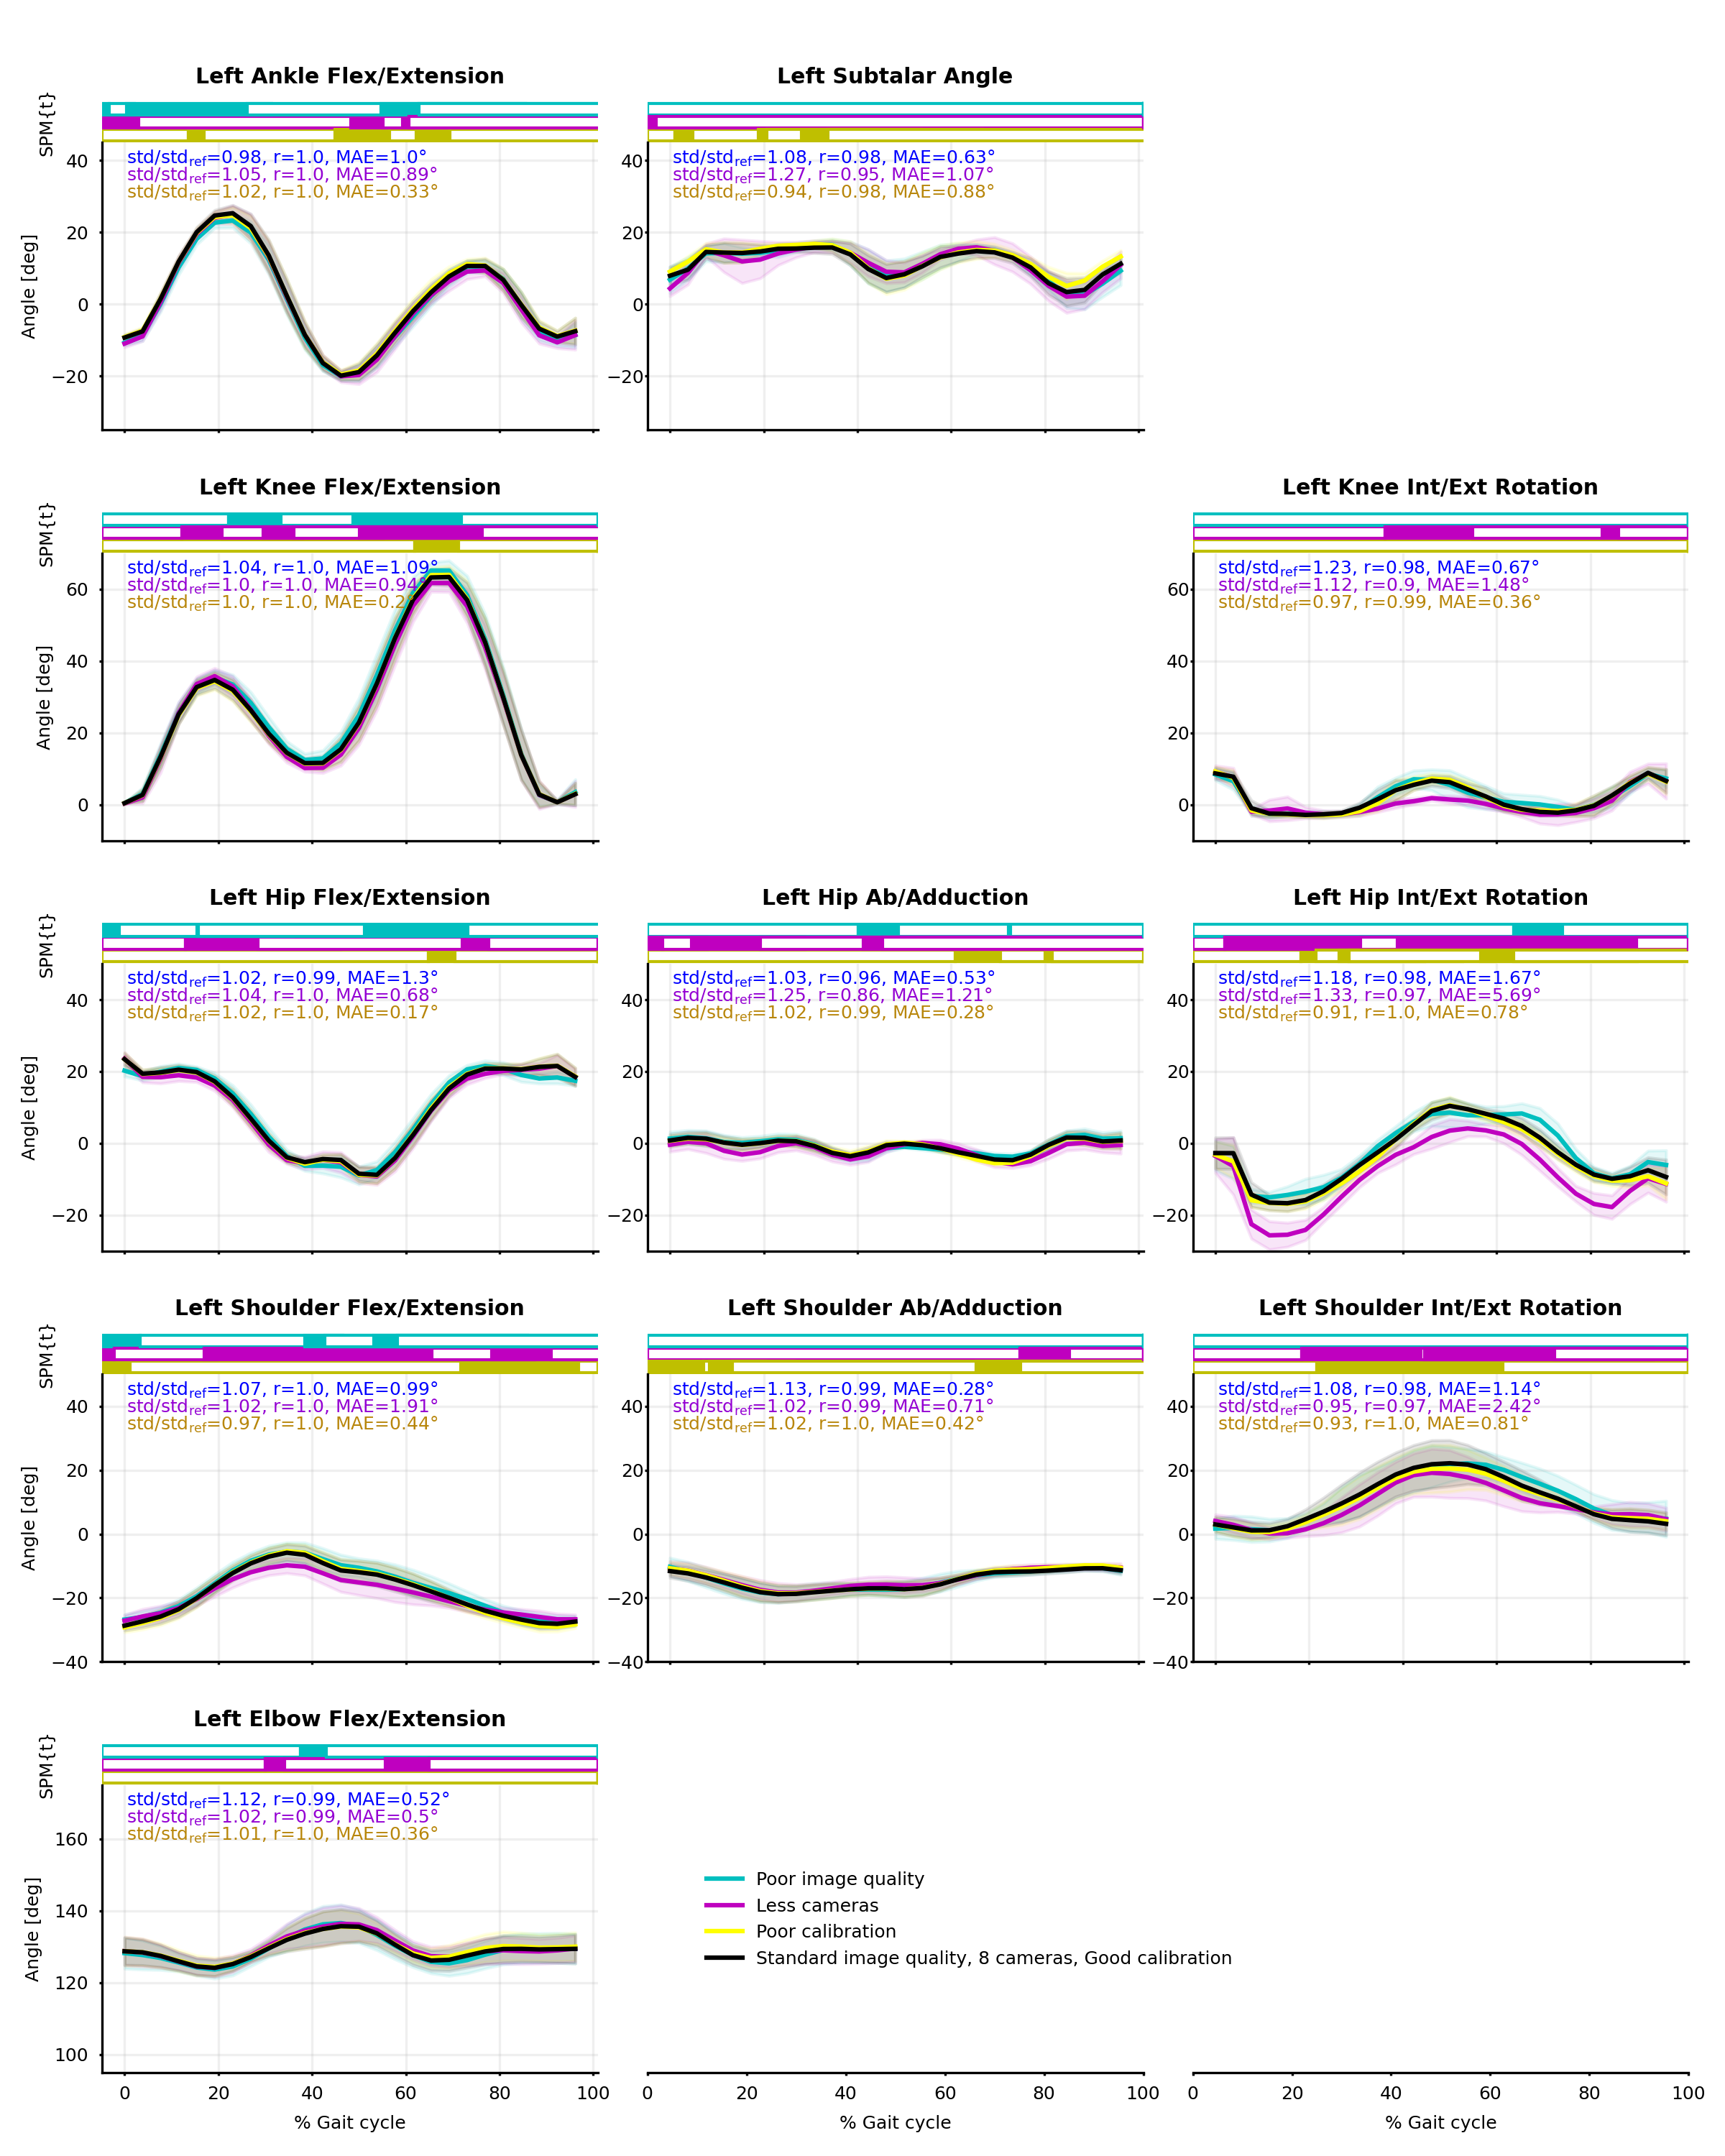
\includegraphics[height=\dimexpr\textheight-145pt]{"../Annexes/Figures/Fig_RunRobust.png"}
	\caption{Joint angle means (solid line) and standard deviations (shaded area) from the nine captured cycles of running. Reference condition (Ref) is black; degraded image quality (Im) is blue; four cameras instead of eight (4c) is purple; degraded calibration (Cal) is yellow. Pearson’s correlation coefficient (r) and mean absolute error (MAE) between Ref and Im, 4c, Cal were calculated. Paired t-tests along time were computed by SPM-1D and are represented as bar plots above the curves: a color rectangle means that there was a cluster of statistically significant differences (\(\alpha\) = 0.05) at that moment.}
	\label{fig_runrobust}
\end{figure}

\clearpage
\section{Robustness: Cycling task results}

\begin{figure}[!ht]
	\centering
	\def\svgwidth{1\columnwidth}
	\fontsize{10pt}{10pt}\selectfont
	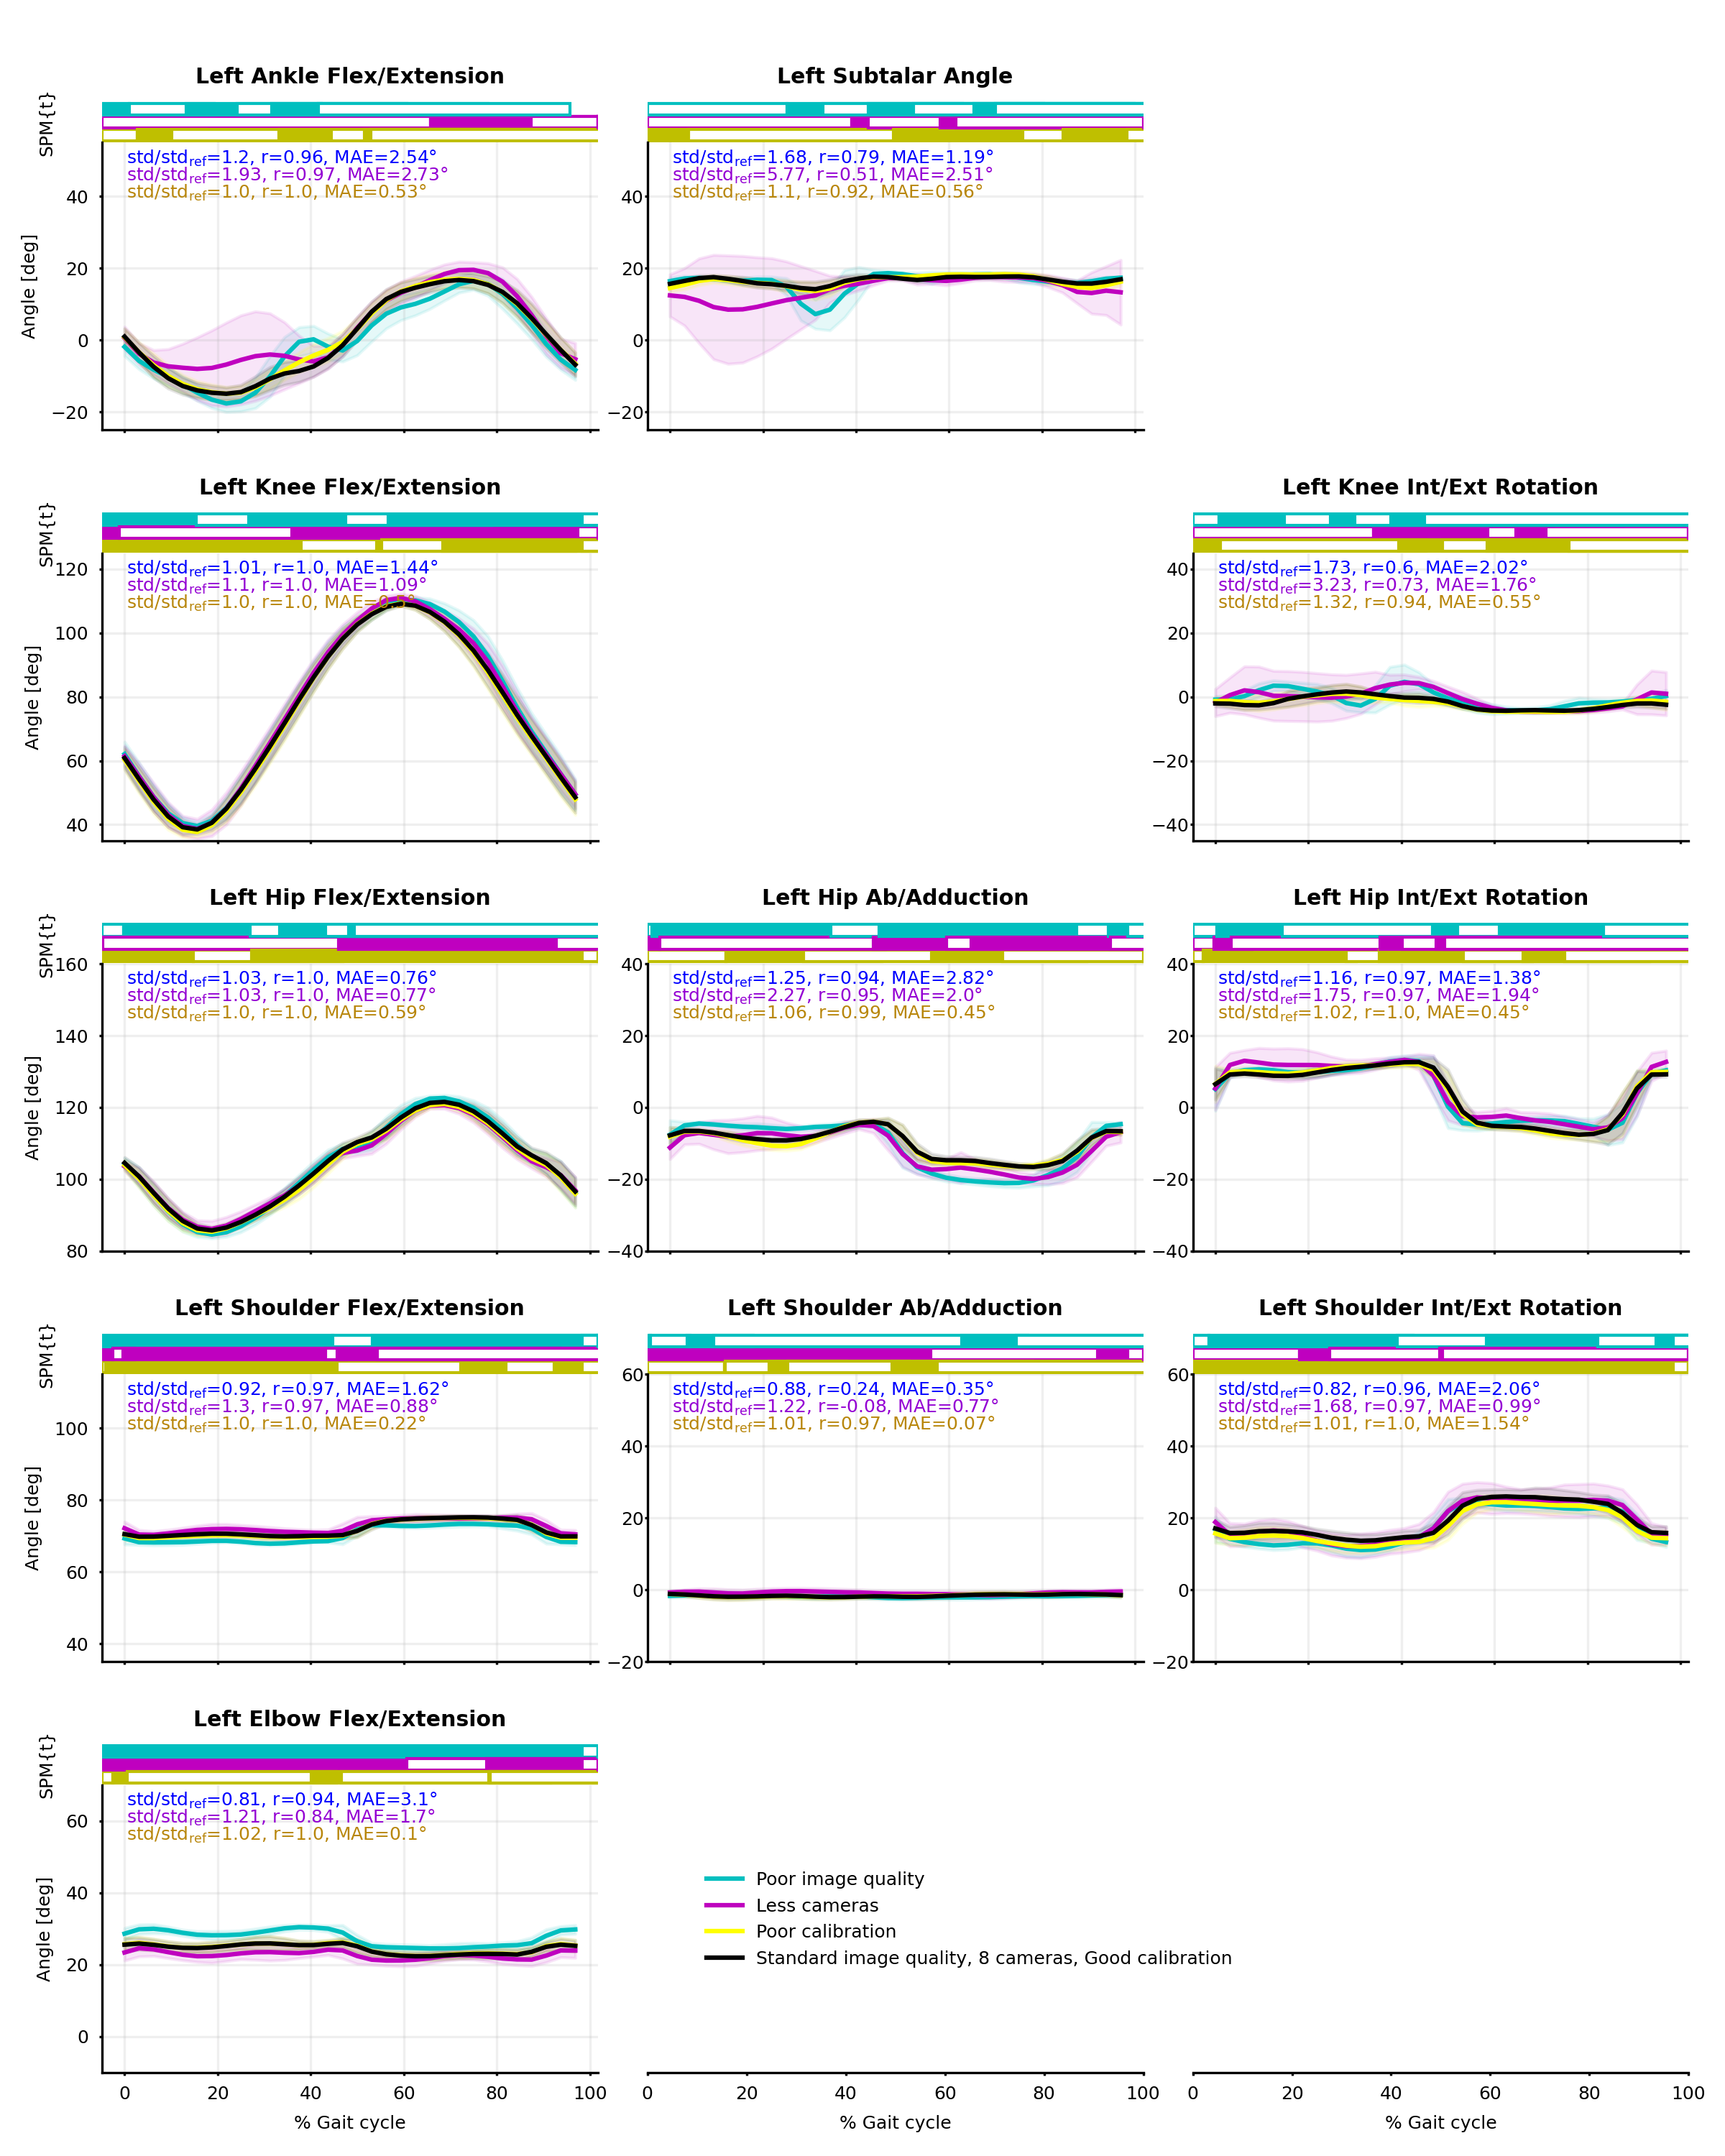
\includegraphics[height=\dimexpr\textheight-145pt]{"../Annexes/Figures/Fig_BikeRobust.png"}
	\caption{Joint angle means (solid line) and standard deviations (shaded area) from the 15 captured cycles of cycling. Reference condition (Ref) is black; degraded image quality (Im) is blue; four cameras instead of eight (4c) is purple; degraded calibration (Cal) is yellow. Pearson’s correlation coefficient (r) and mean absolute error (MAE) between Ref and Im, 4c, Cal were calculated. Paired t-tests along time were computed by SPM-1D and are represented as bar plots above the curves: a color rectangle means that there was a cluster of statistically significant differences (\(\alpha\) = 0.05) at that moment.}
	\label{fig_bikerobust}
\end{figure}


\FloatBarrier
\chapter{Appendix B on Accuracy assessment}
\label{Ann:2}

%==============================================================================	Résumé du chapitre

\begin{center}
\rule{0.7\linewidth}{.5pt}
\begin{minipage}{0.7\linewidth}
\smallskip

\textit{
Supplementary figures for Chapter 5 on \nameref{ch:5}, for the lower-body analysis of the running and cycling tasks, and for the upper-body analysis of all three tasks. \newline\newline All details on methods and results on the lower-body are provided in the forementioned chapter. Results and discussion on the upper-body are debated section \ref{upper_acc}.
}

%\smallskip
\end{minipage}
\smallskip
\rule{0.7\linewidth}{.5pt}
\end{center}

\minitoc
\newpage

\section{Lower-body results for the running and cycling tasks}

Lower-body graphs are provided on Figure~\ref{fig_qtmrun} and on Figure~\ref{fig_blandrun} for the running task, and on Figure~\ref{fig_qtmbike} and on Figure~\ref{fig_blandbike}. However, all results are discussed in the main body of the article on \nameref{ch:5}.

\subsection{Accuracy: Running task results}

\begin{figure}[!ht]
	\centering
	\def\svgwidth{1\columnwidth}
	\fontsize{10pt}{10pt}\selectfont
	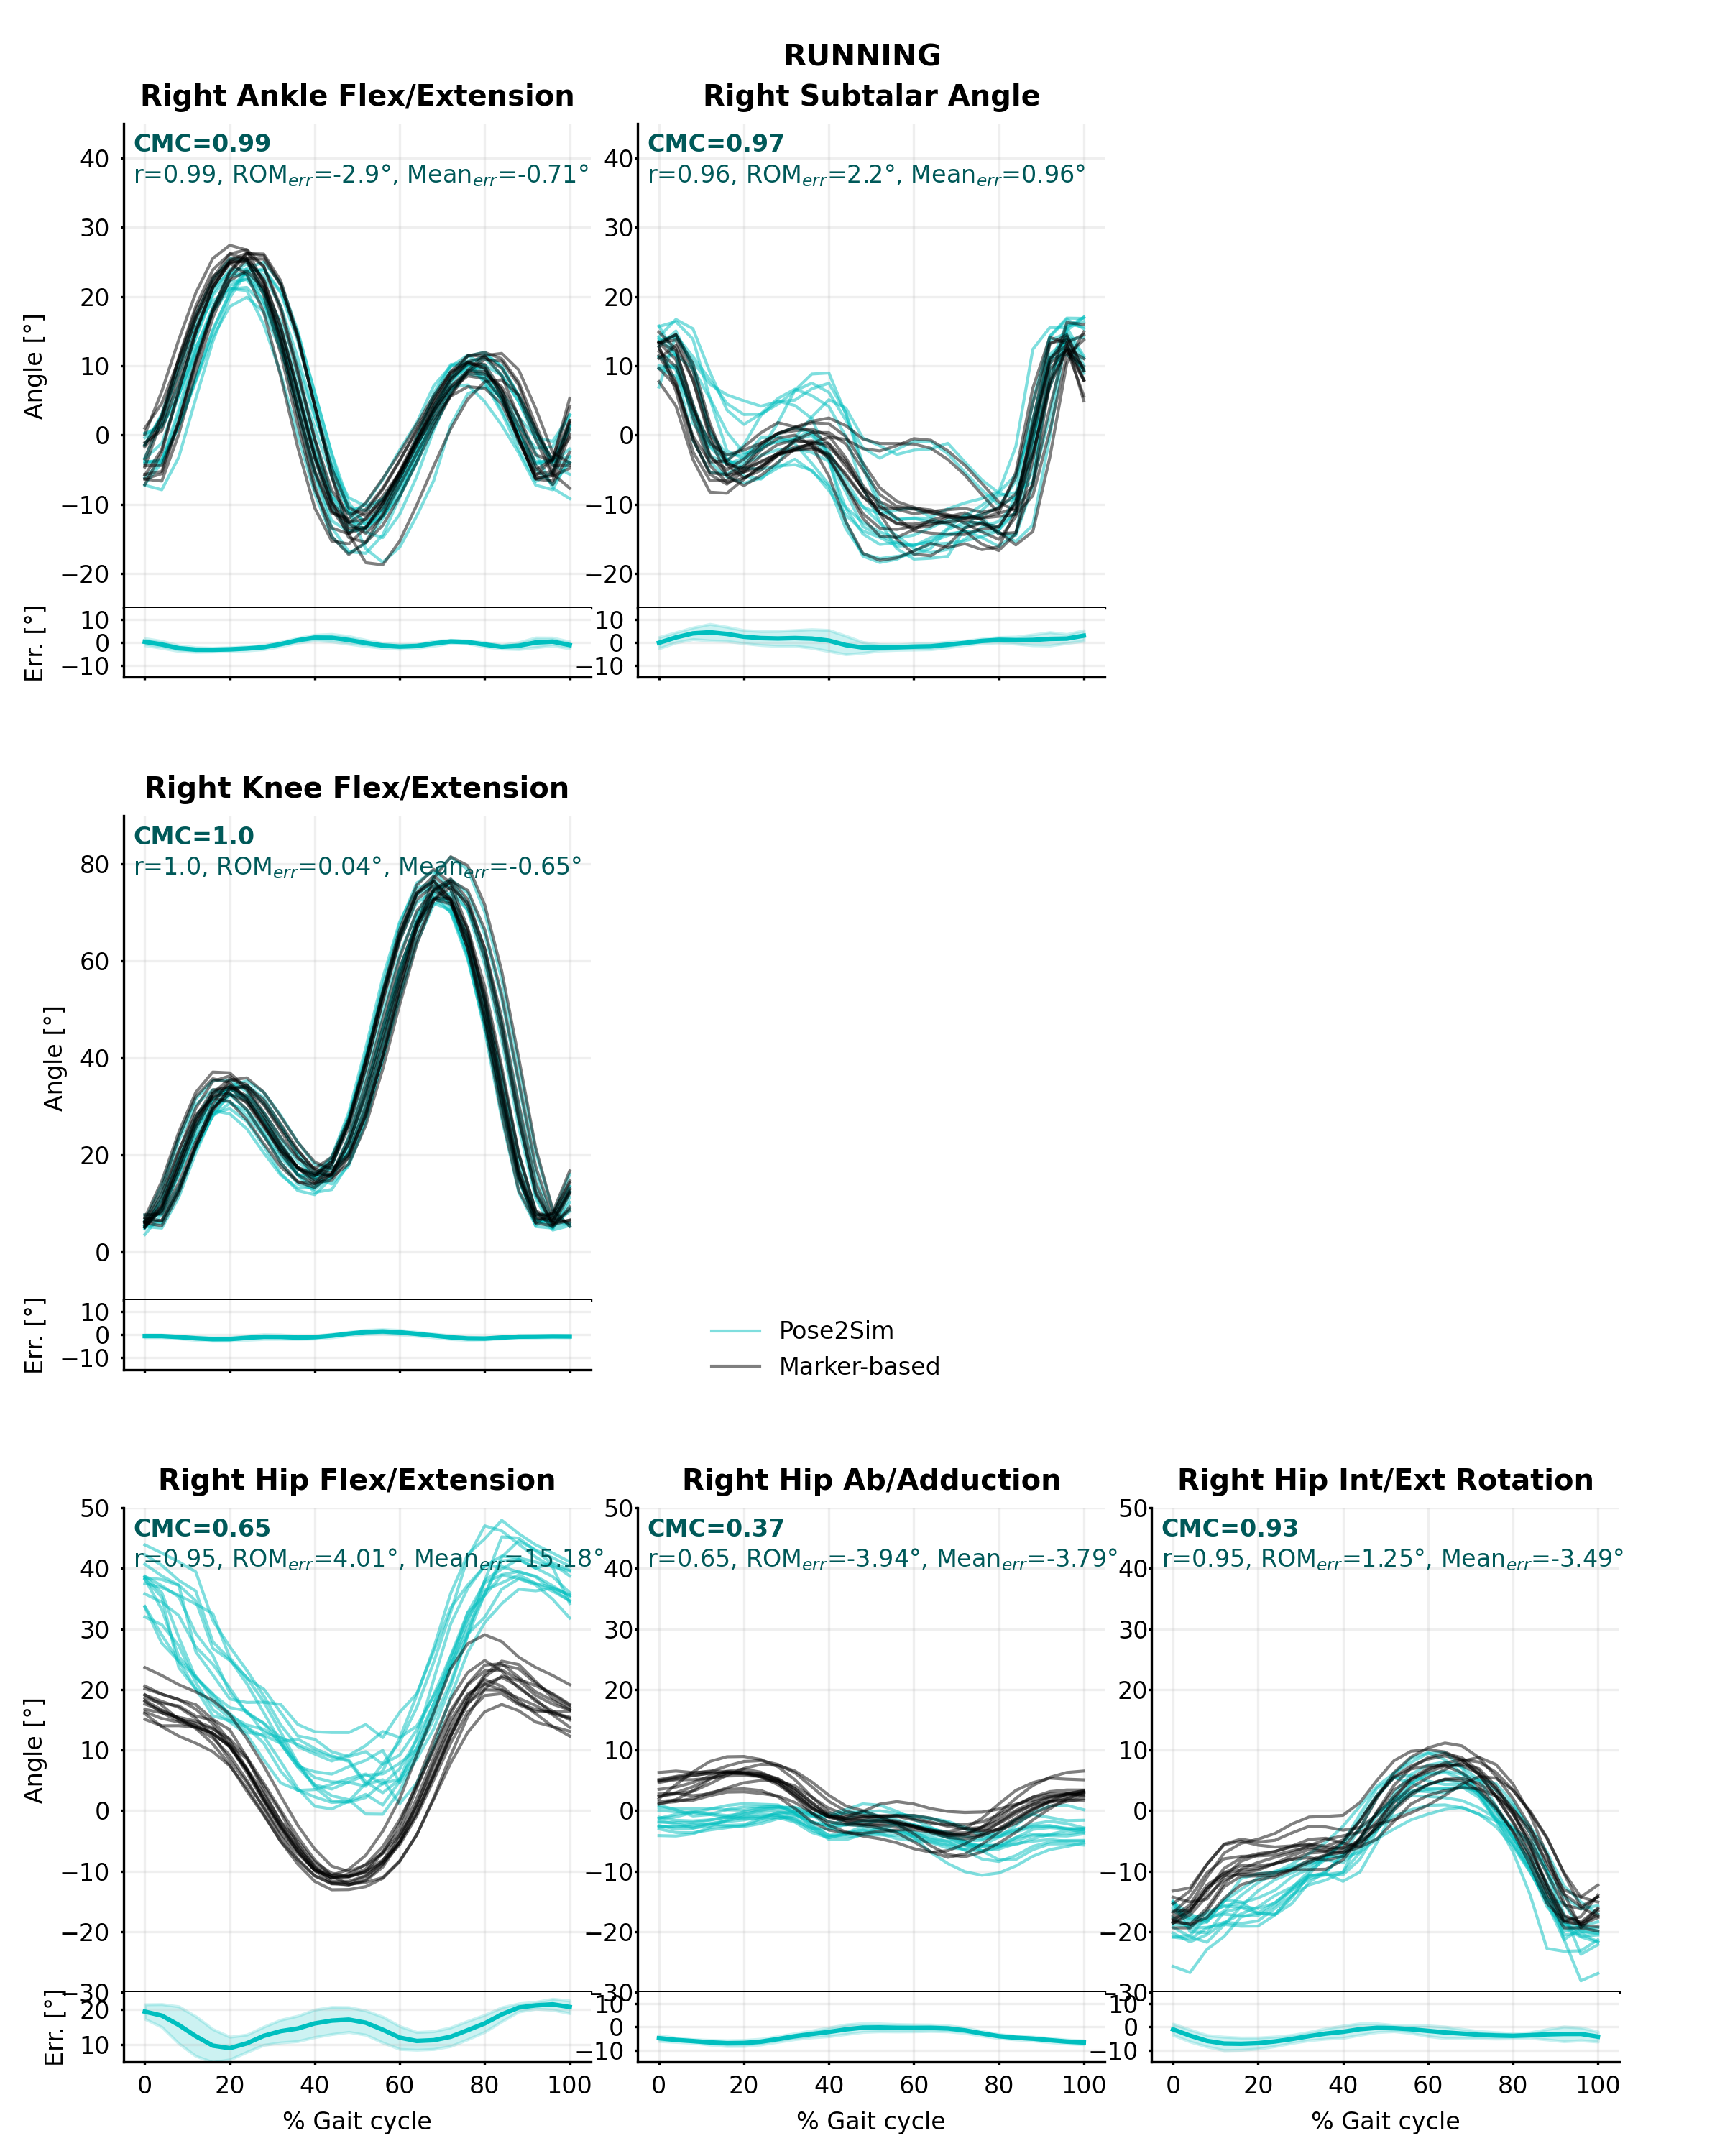
\includegraphics[width=.94\linewidth]{"../Annexes/Figures/Fig_QTMRun.png"}
	\caption{Pose2Sim (cyan) and marker-based (black) lower-body joint angles for the running task. Coefficient of multiple correlation (CMC) is indicated, and broken down into, respectively, Pearson’s coefficient (r) for correlation assessment, range of motion errors (\(ROM_{err}\)) for gain, and overall mean errors (\(Mean_{err}\)) for offset. Mean error and standard deviations are also represented at the bottom of the graphics.}
	\label{fig_qtmrun}
\end{figure}

\begin{figure}[!ht]
	\centering
	\def\svgwidth{1\columnwidth}
	\fontsize{10pt}{10pt}\selectfont
	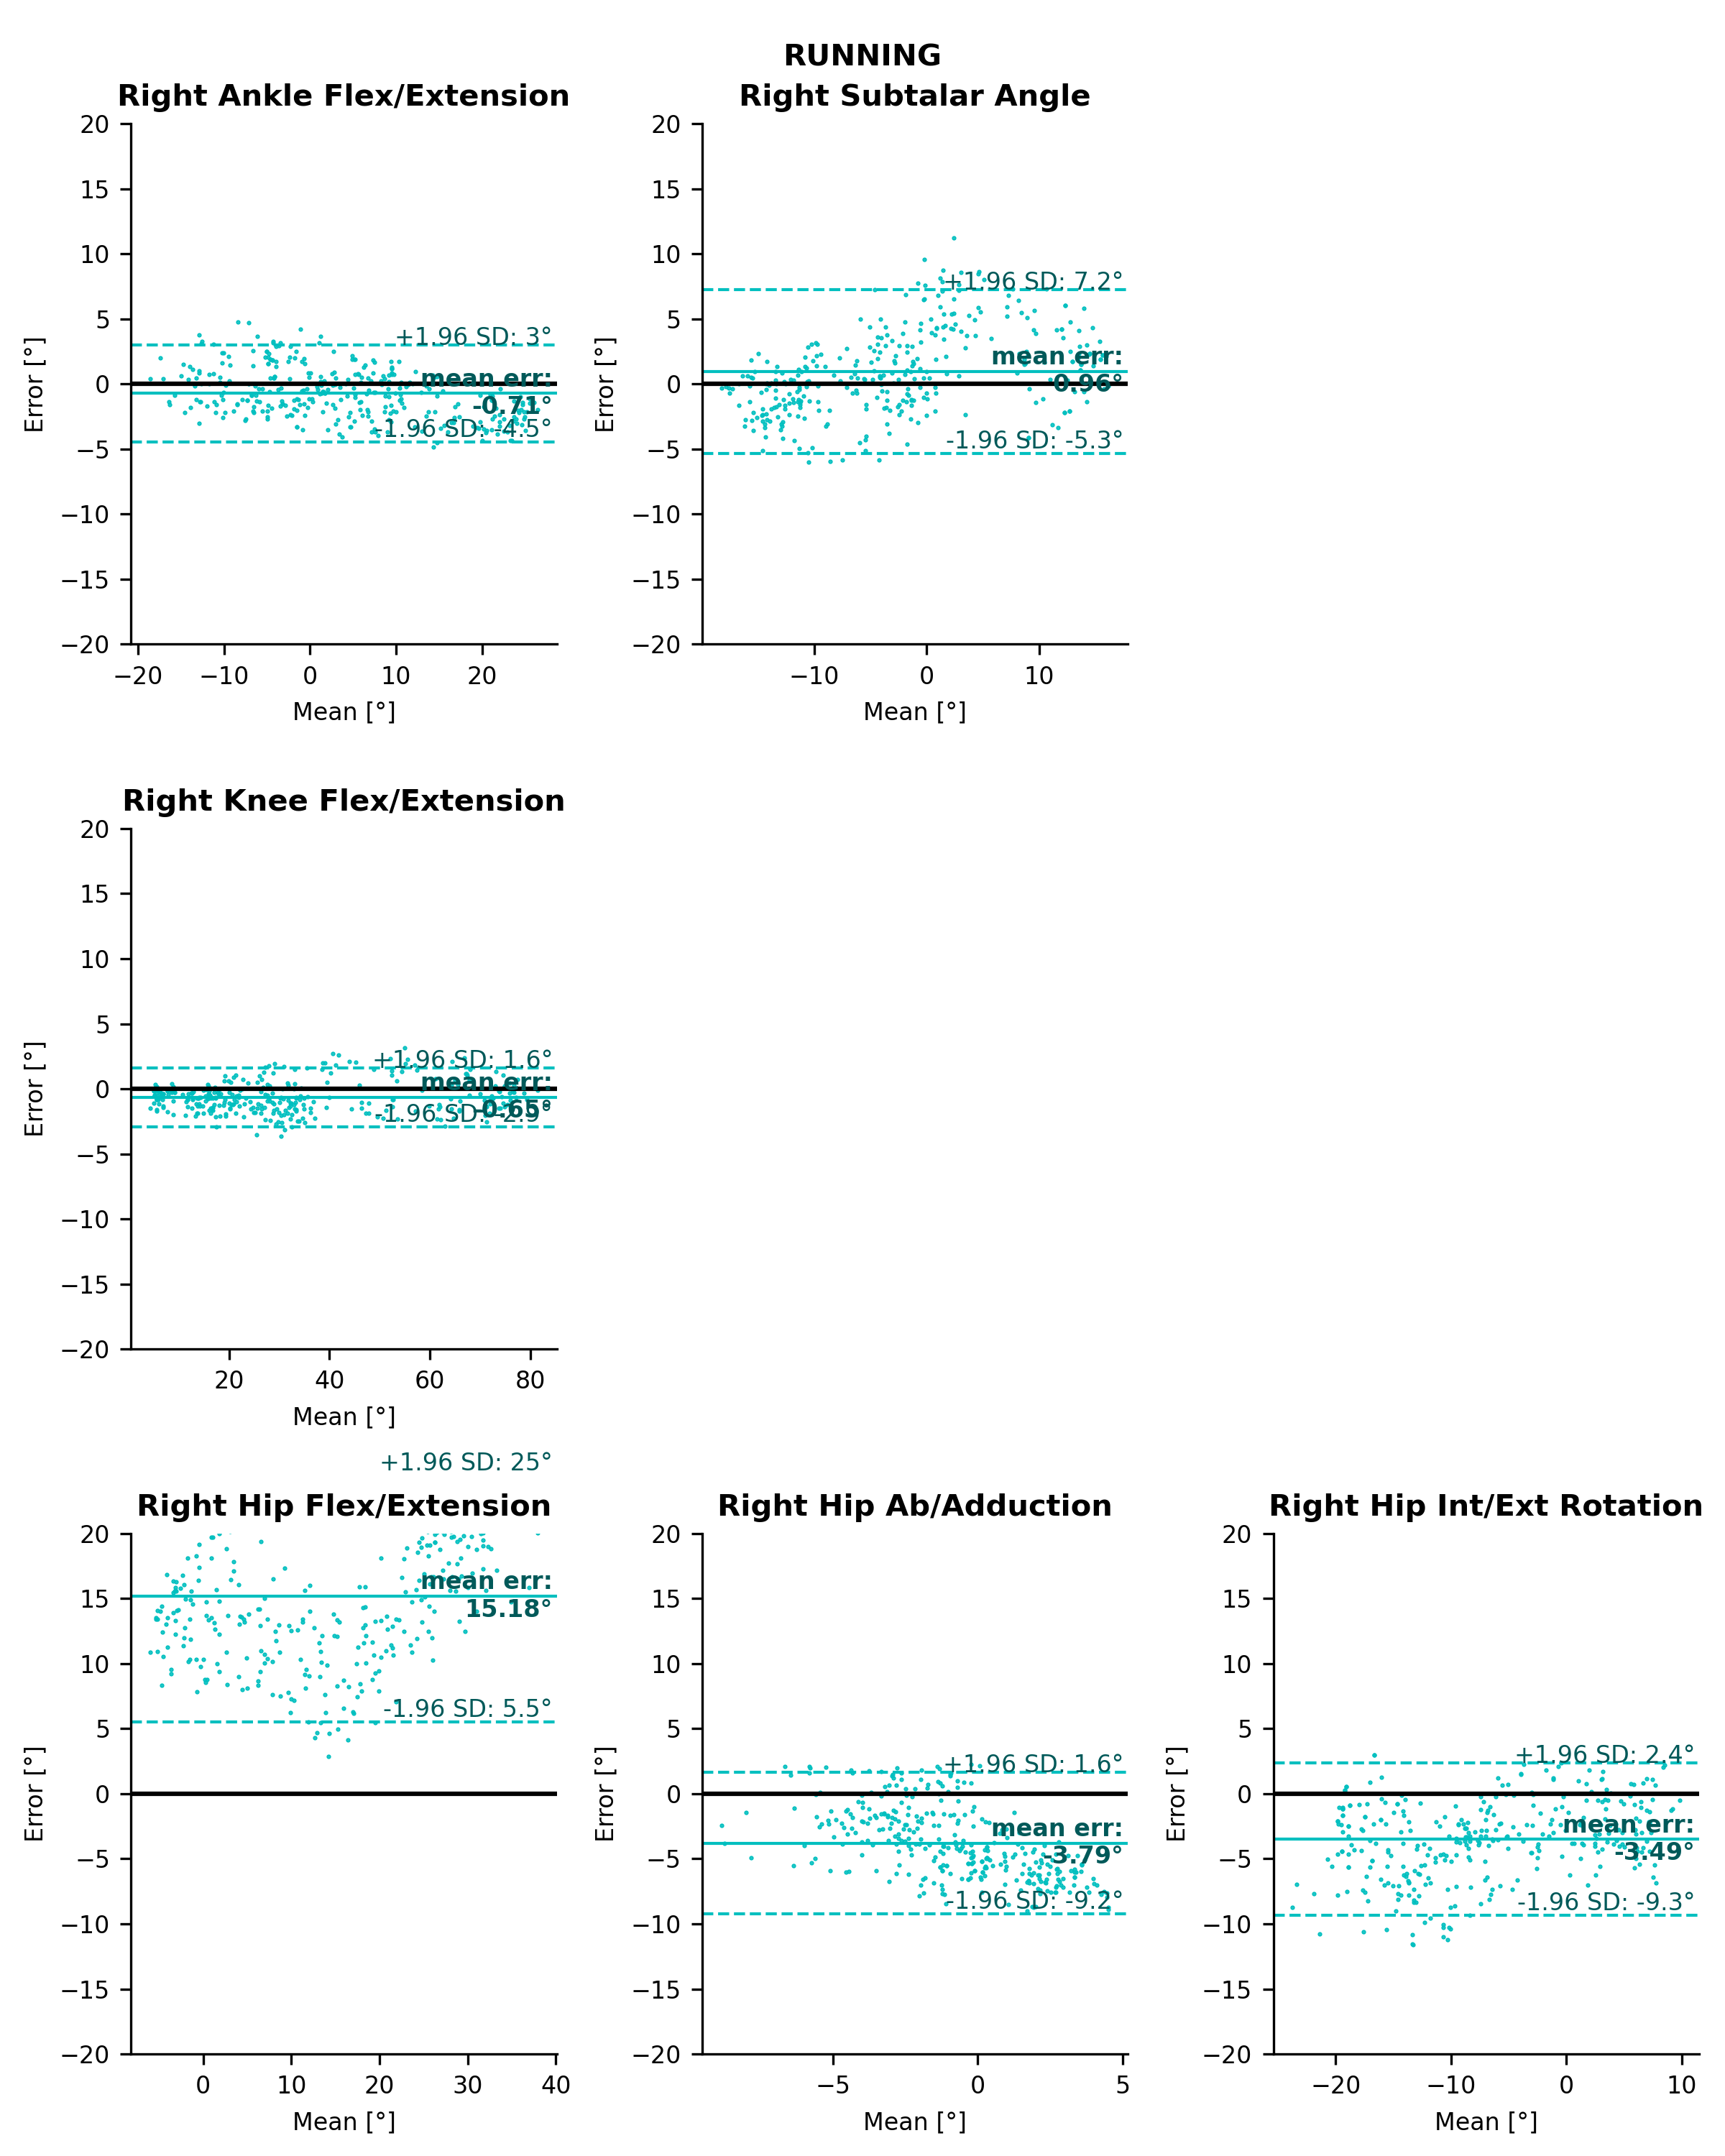
\includegraphics[height=\dimexpr\textheight-119pt]{"../Annexes/Figures/Fig_BlandRun.png"}
	\caption{Bland–Altman analysis of lower-body joint angle errors for the running task. Mean bias is represented as a horizontal solid, bold line, and 95\% limits of agreement are represented as dotted lines.}
	\label{fig_blandrun}
\end{figure}


\clearpage
\subsection{Accuracy: Cycling task results}

\begin{figure}[!ht]
	\centering
	\def\svgwidth{1\columnwidth}
	\fontsize{10pt}{10pt}\selectfont
	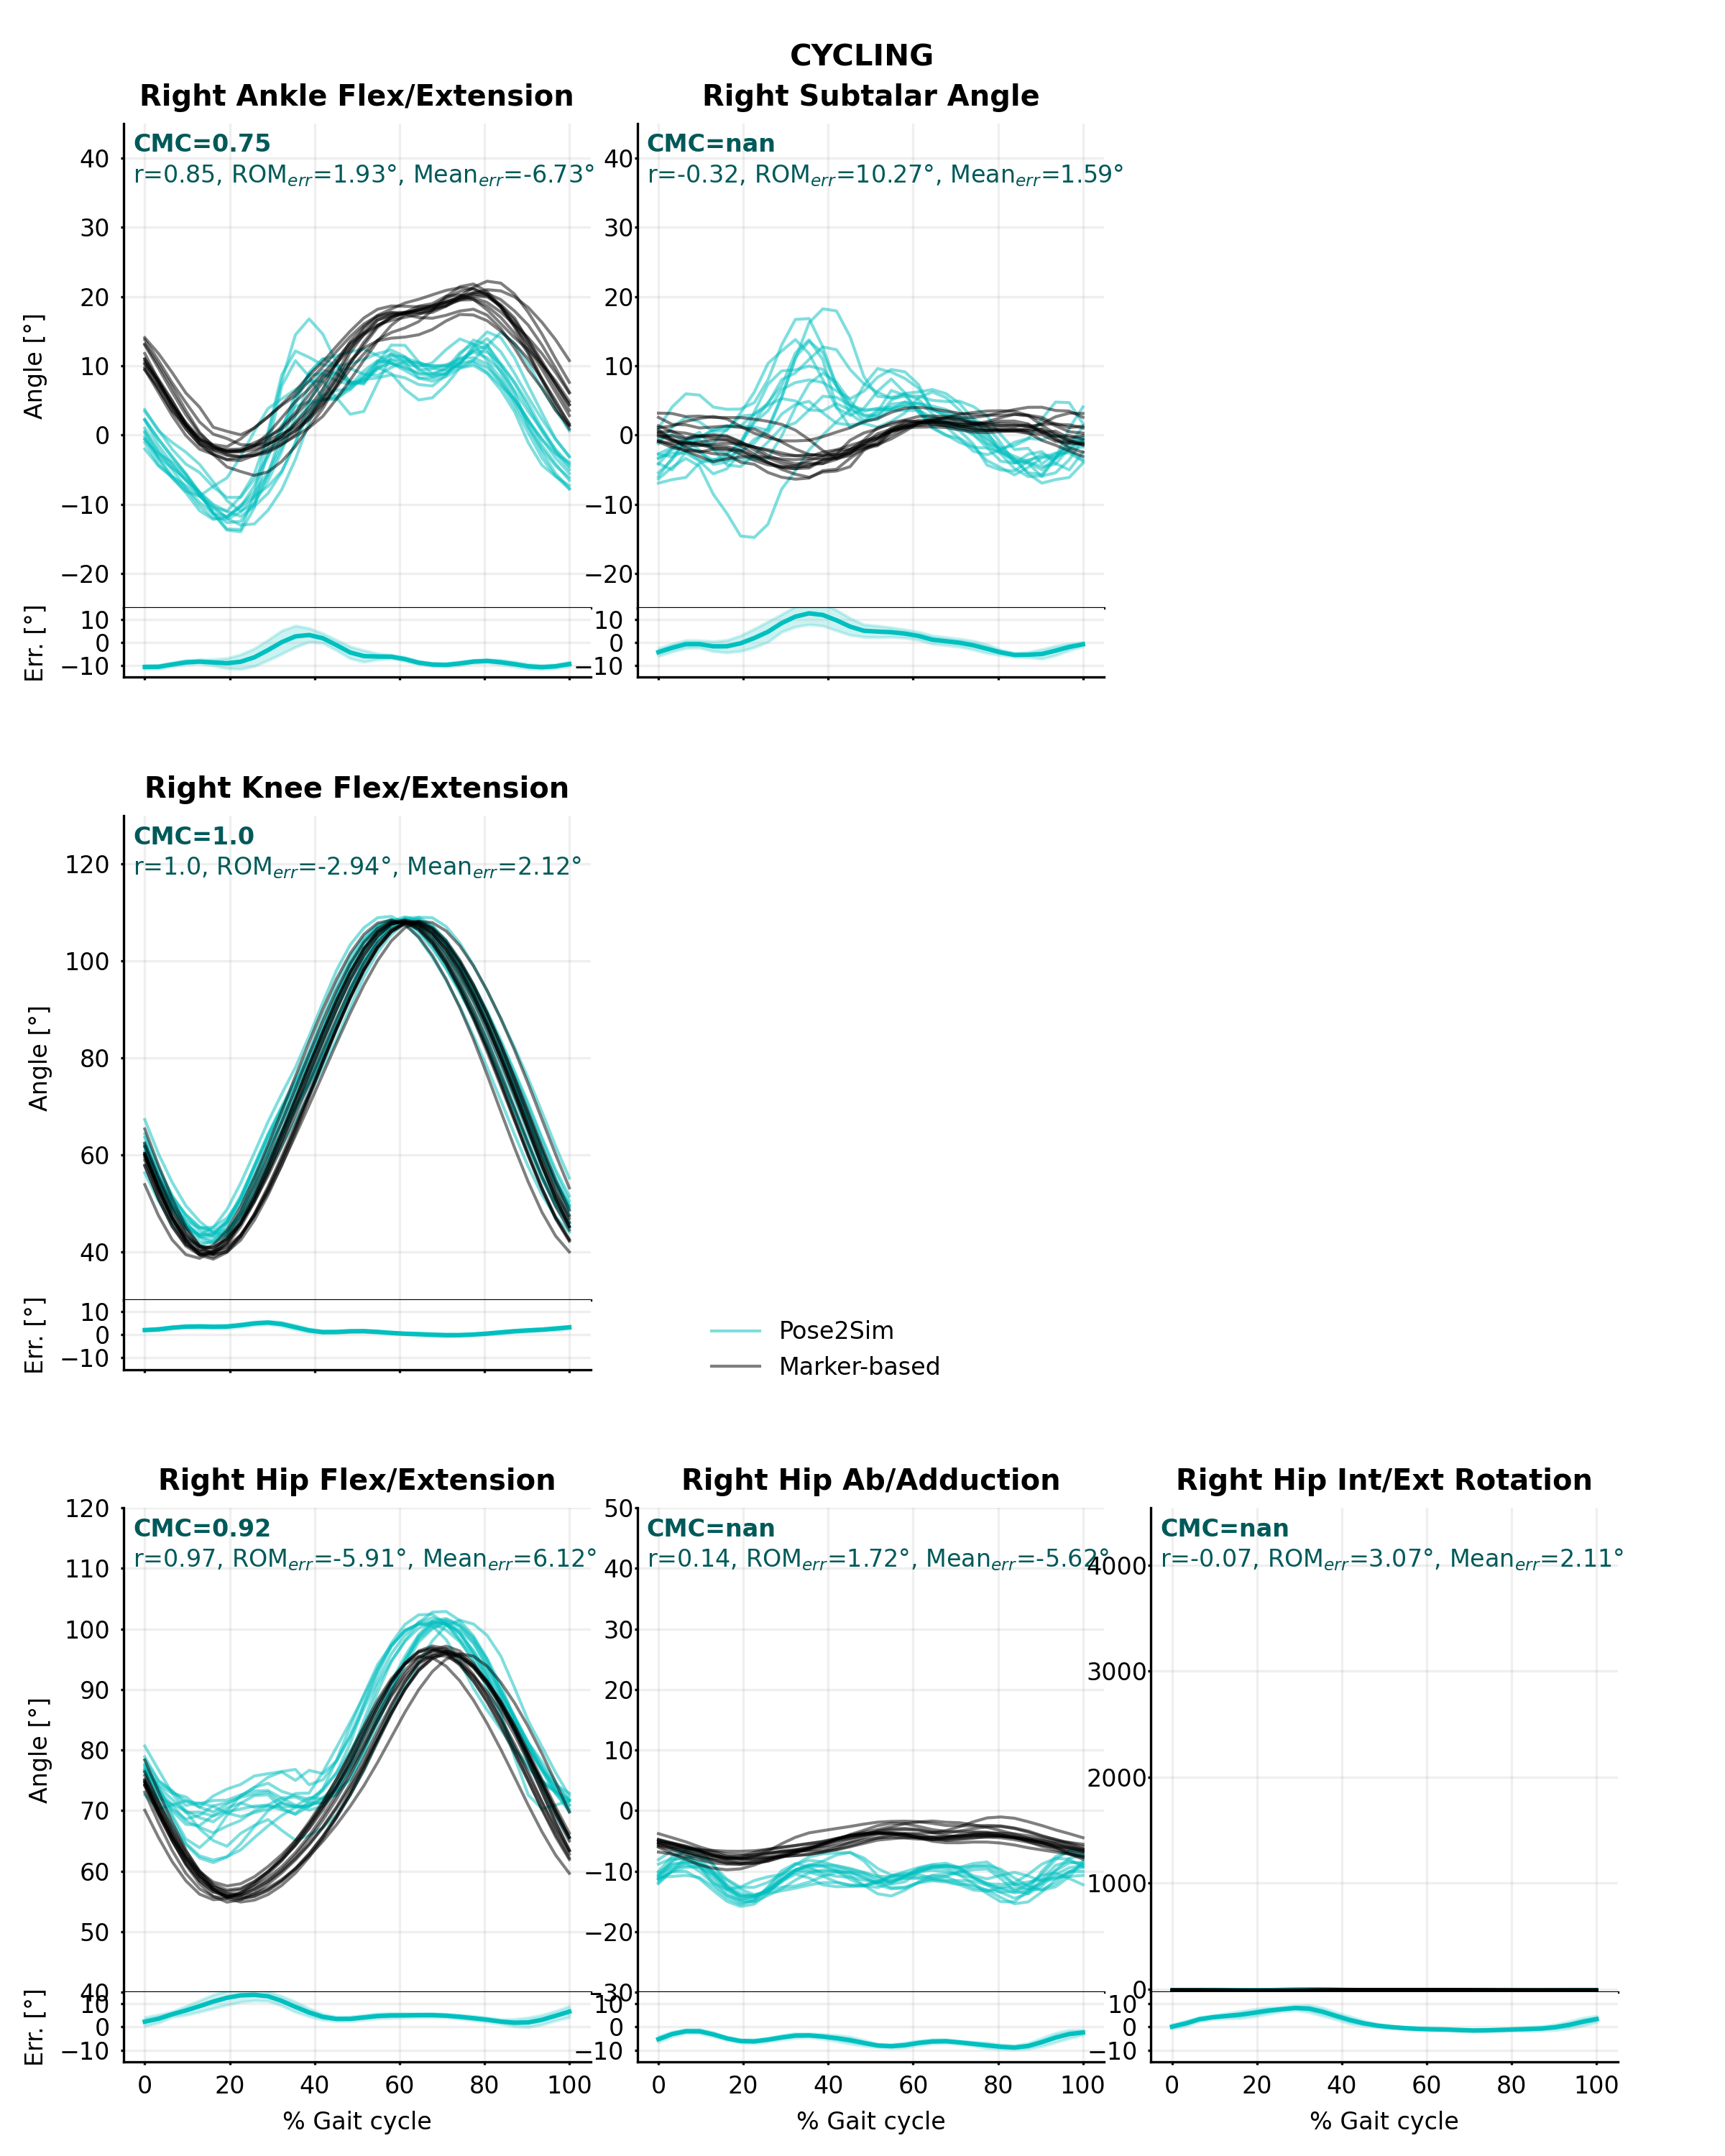
\includegraphics[height=\dimexpr\textheight-119pt]{"../Annexes/Figures/Fig_QTMBike.png"}
	\caption{Pose2Sim (cyan) and marker-based (black) lower-body joint angles for the cycling task. Coefficient of multiple correlation (CMC) is indicated, and broken down into, respectively, Pearson’s coefficient (r) for correlation assessment, range of motion errors (\(ROM_{err}\)) for gain, and overall mean errors (\(Mean_{err}\)) for offset. Mean error and standard deviations are also represented at the bottom of the graphics.}
	\label{fig_qtmbike}
\end{figure}

\begin{figure}[!ht]
	\centering
	\def\svgwidth{1\columnwidth}
	\fontsize{10pt}{10pt}\selectfont
	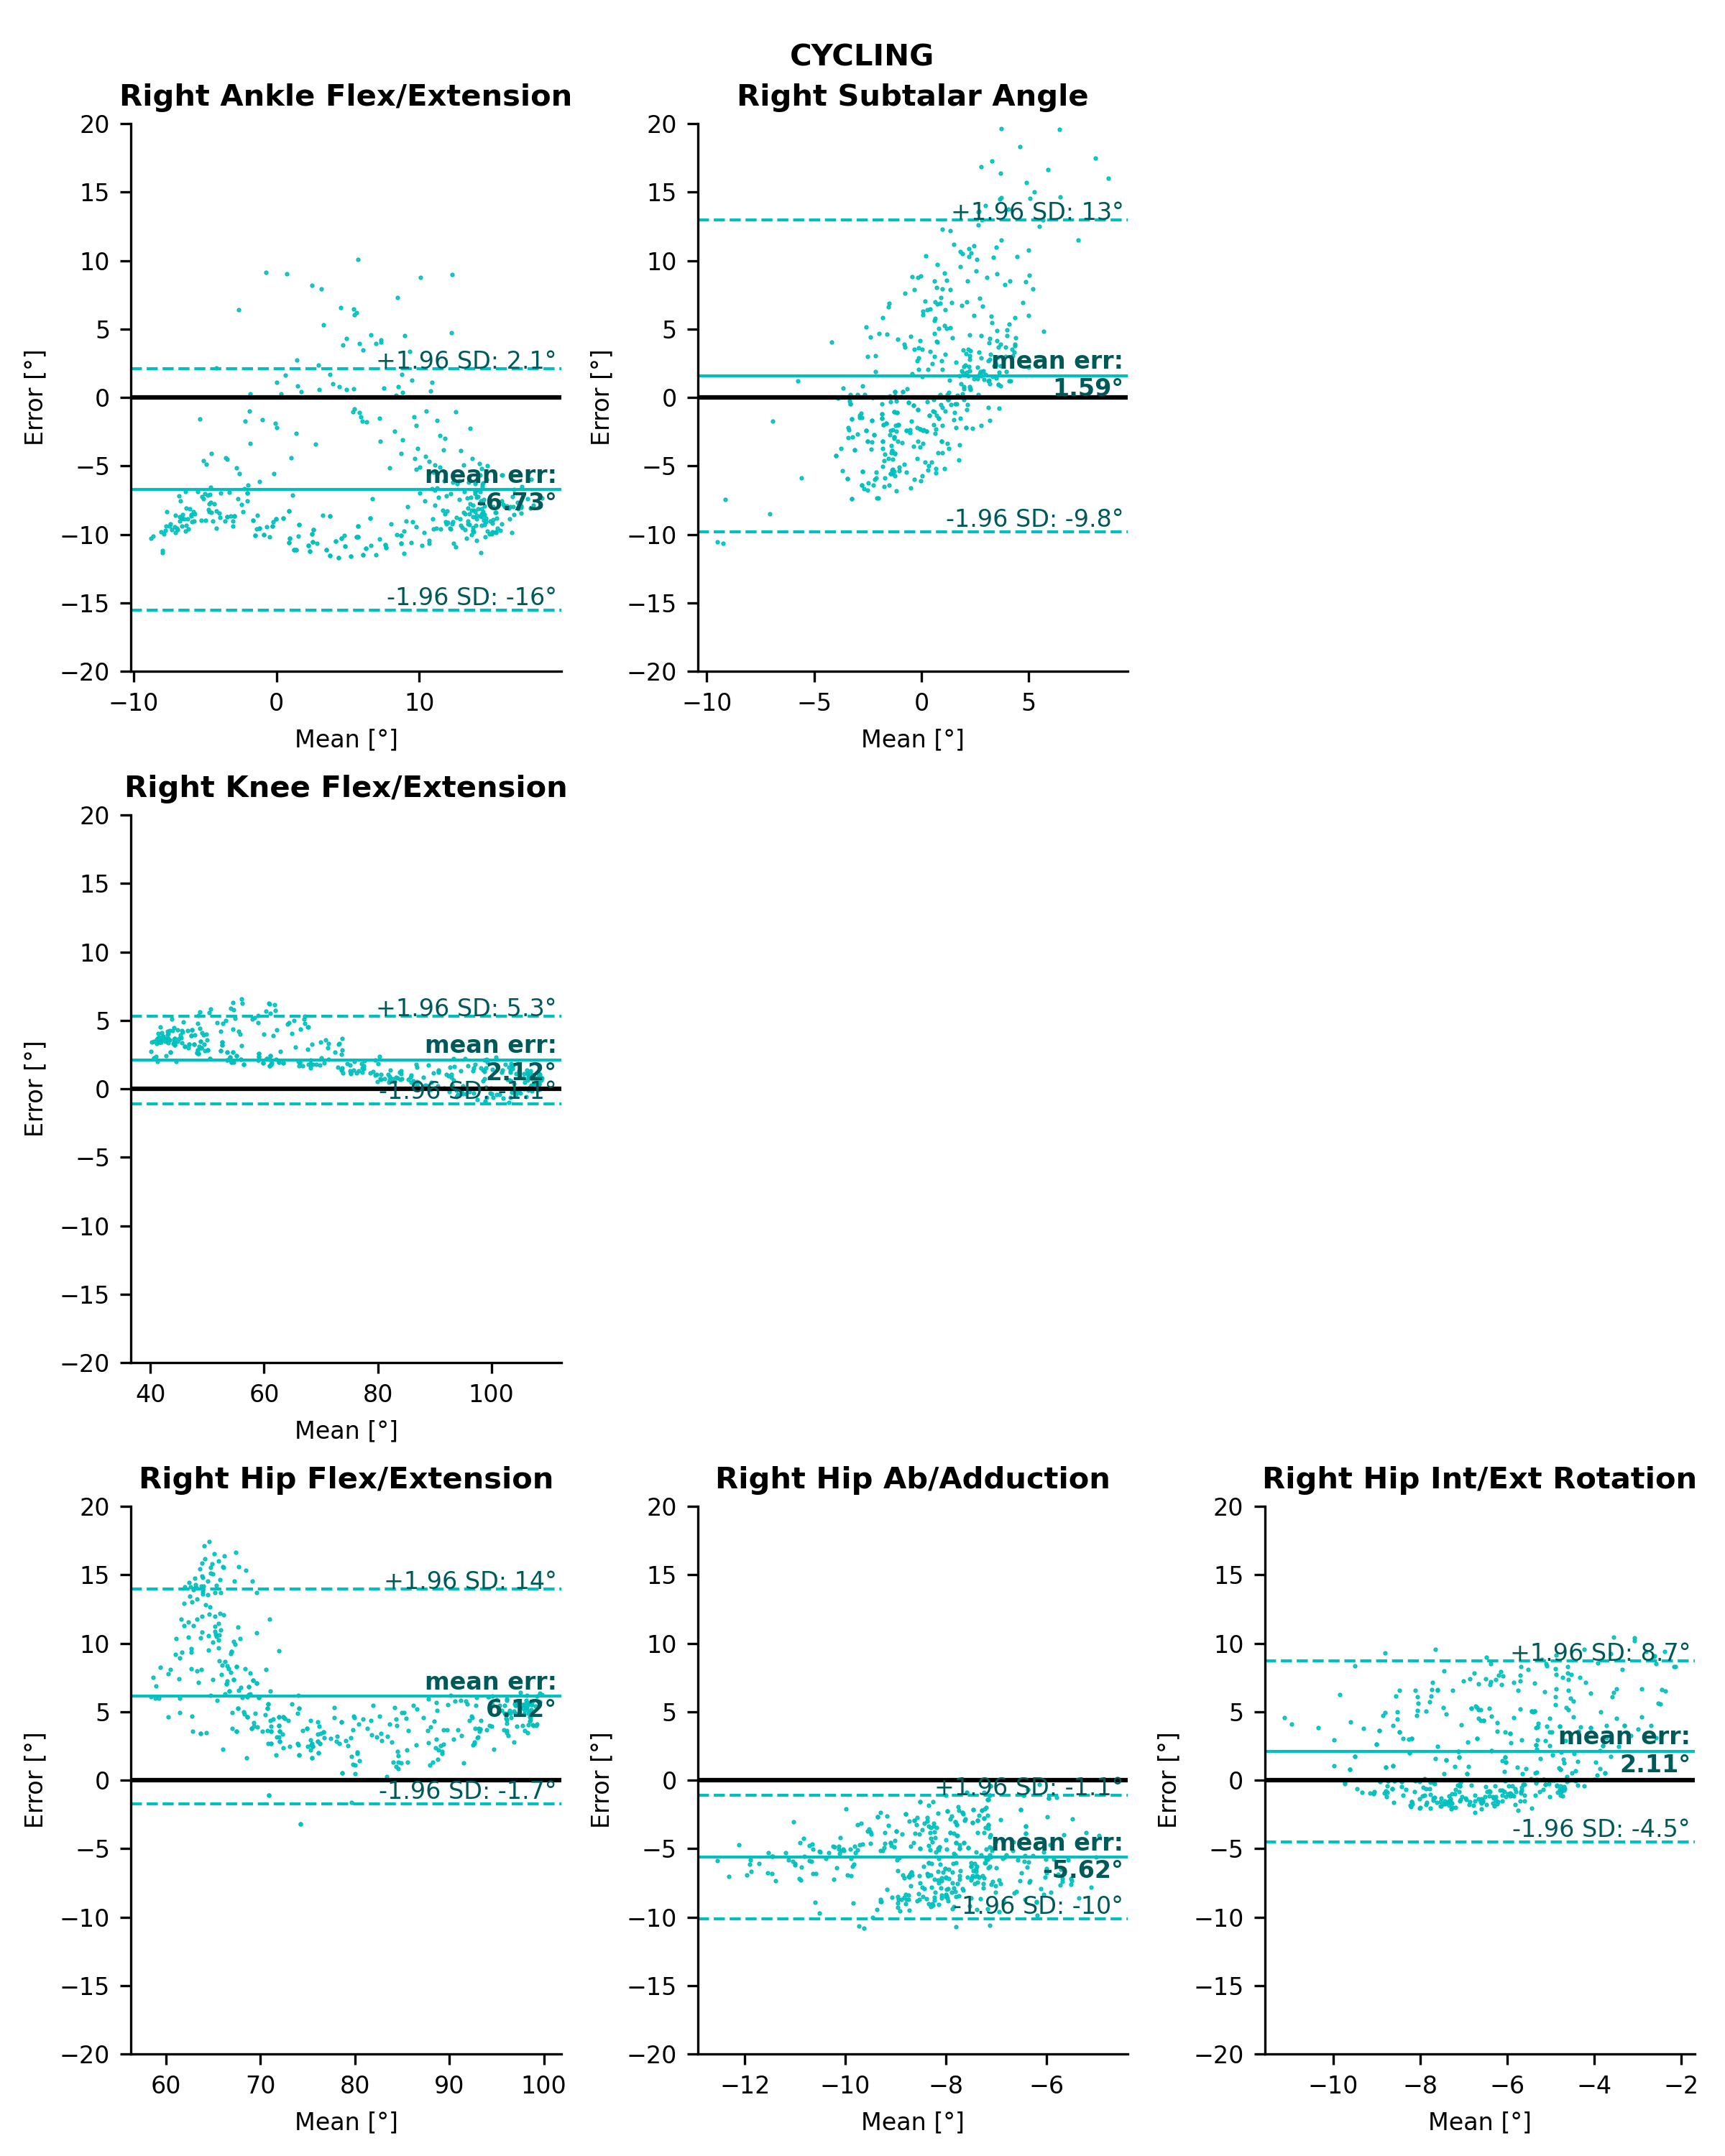
\includegraphics[height=\dimexpr\textheight-119pt]{"../Annexes/Figures/Fig_BlandBike.png"}
	\caption{Bland–Altman analysis of lower-body joint angle errors for the cycling task. Mean bias is represented as a horizontal solid, bold line, and 95\% limits of agreement are represented as dotted lines.}
	\label{fig_blandbike}
\end{figure}

\clearpage

\section{Sacro-lumbar and upper-body results for all tasks}\label{upper_acc}

Although the article focused on lower limb kinematics, we ran the same analysis on sacro-lumbar, elbow, and shoulder joints for all three tasks (Figure~\ref{fig_qtmwalkup} and Figure~\ref{fig_blandwalkup} for walking, Figure~\ref{fig_qtmrunup} and Figure~\ref{fig_blandrunup} for running, and Figure~\ref{fig_qtmbikeup} and Figure~\ref{fig_blandbikeup} for cycling). The OpenPose model we used does not allow for the capture of wrist deviation or pronation/supination, or of any hand or finger movement.

Results were generally less good than in the lower body, especially on sacro-lumbar flexion/extension, for which all CMC values were complex. This can be attributed both to the lack of OpenPose keypoints in this area, and to the simplicity of the OpenSim model in the upper-body part. Indeed, currently all pelvis, lumbar, and thoracic angles are solely determined by the detection of the hip keypoints on the lower part, and of the shoulder and neck keypoints on the upper part. Moreover, the skeletal model did not allow for any scapulo-thoracic degree of freedom. In addition to the sacro-lumbar joint, upper-body Pearson’s correlation coefficients were mostly very good (>0.85) in most planes in walking and running. The range of motion error remained below 1° for shoulder and elbow angles in walking, while it reached almost 5° in the shoulder and 2° in the elbow in running. The mean error in the sagittal plane was below 1° in the shoulder angle in walking, but it reached 10° in the elbow; conversely, in running it reached 9° in the shoulder but remained under 1° in the elbow. In cycling, upper-body Pose2Sim angles were mostly not correlated to marker-based ones, and ROM errors and mean errors were much worse than in other tasks. Moreover, the Bland–Altman analysis showed that the data is heteroscedastic: the spread and magnitude of the errors varied as the joint angle evolved.

In conclusion, Pose2Sim does not evaluate some anatomical joint angles in the upper body, and is generally less accurate than for the lower body. This is mostly due to the lack of keypoints OpenPose detects. To date, OpenPose offers hand and face models but no detailed model of the upper limb exists. Pose2Sim could be used with other pose estimation algorithms, including custom ones leveraging DeepLabCut \cite{Mathis2018,Lauer2022}, for example, although it would involve manually labeling a large training dataset. This would enable the use of a more anatomically realistic kinematic model, such as the one proposed by \cite{Seth2016} for the shoulder girdle.

\clearpage
\subsection{Accuracy: Upper-body results for the walking task}

\begin{figure}[!ht]
	\centering
	\def\svgwidth{1\columnwidth}
	\fontsize{10pt}{10pt}\selectfont
	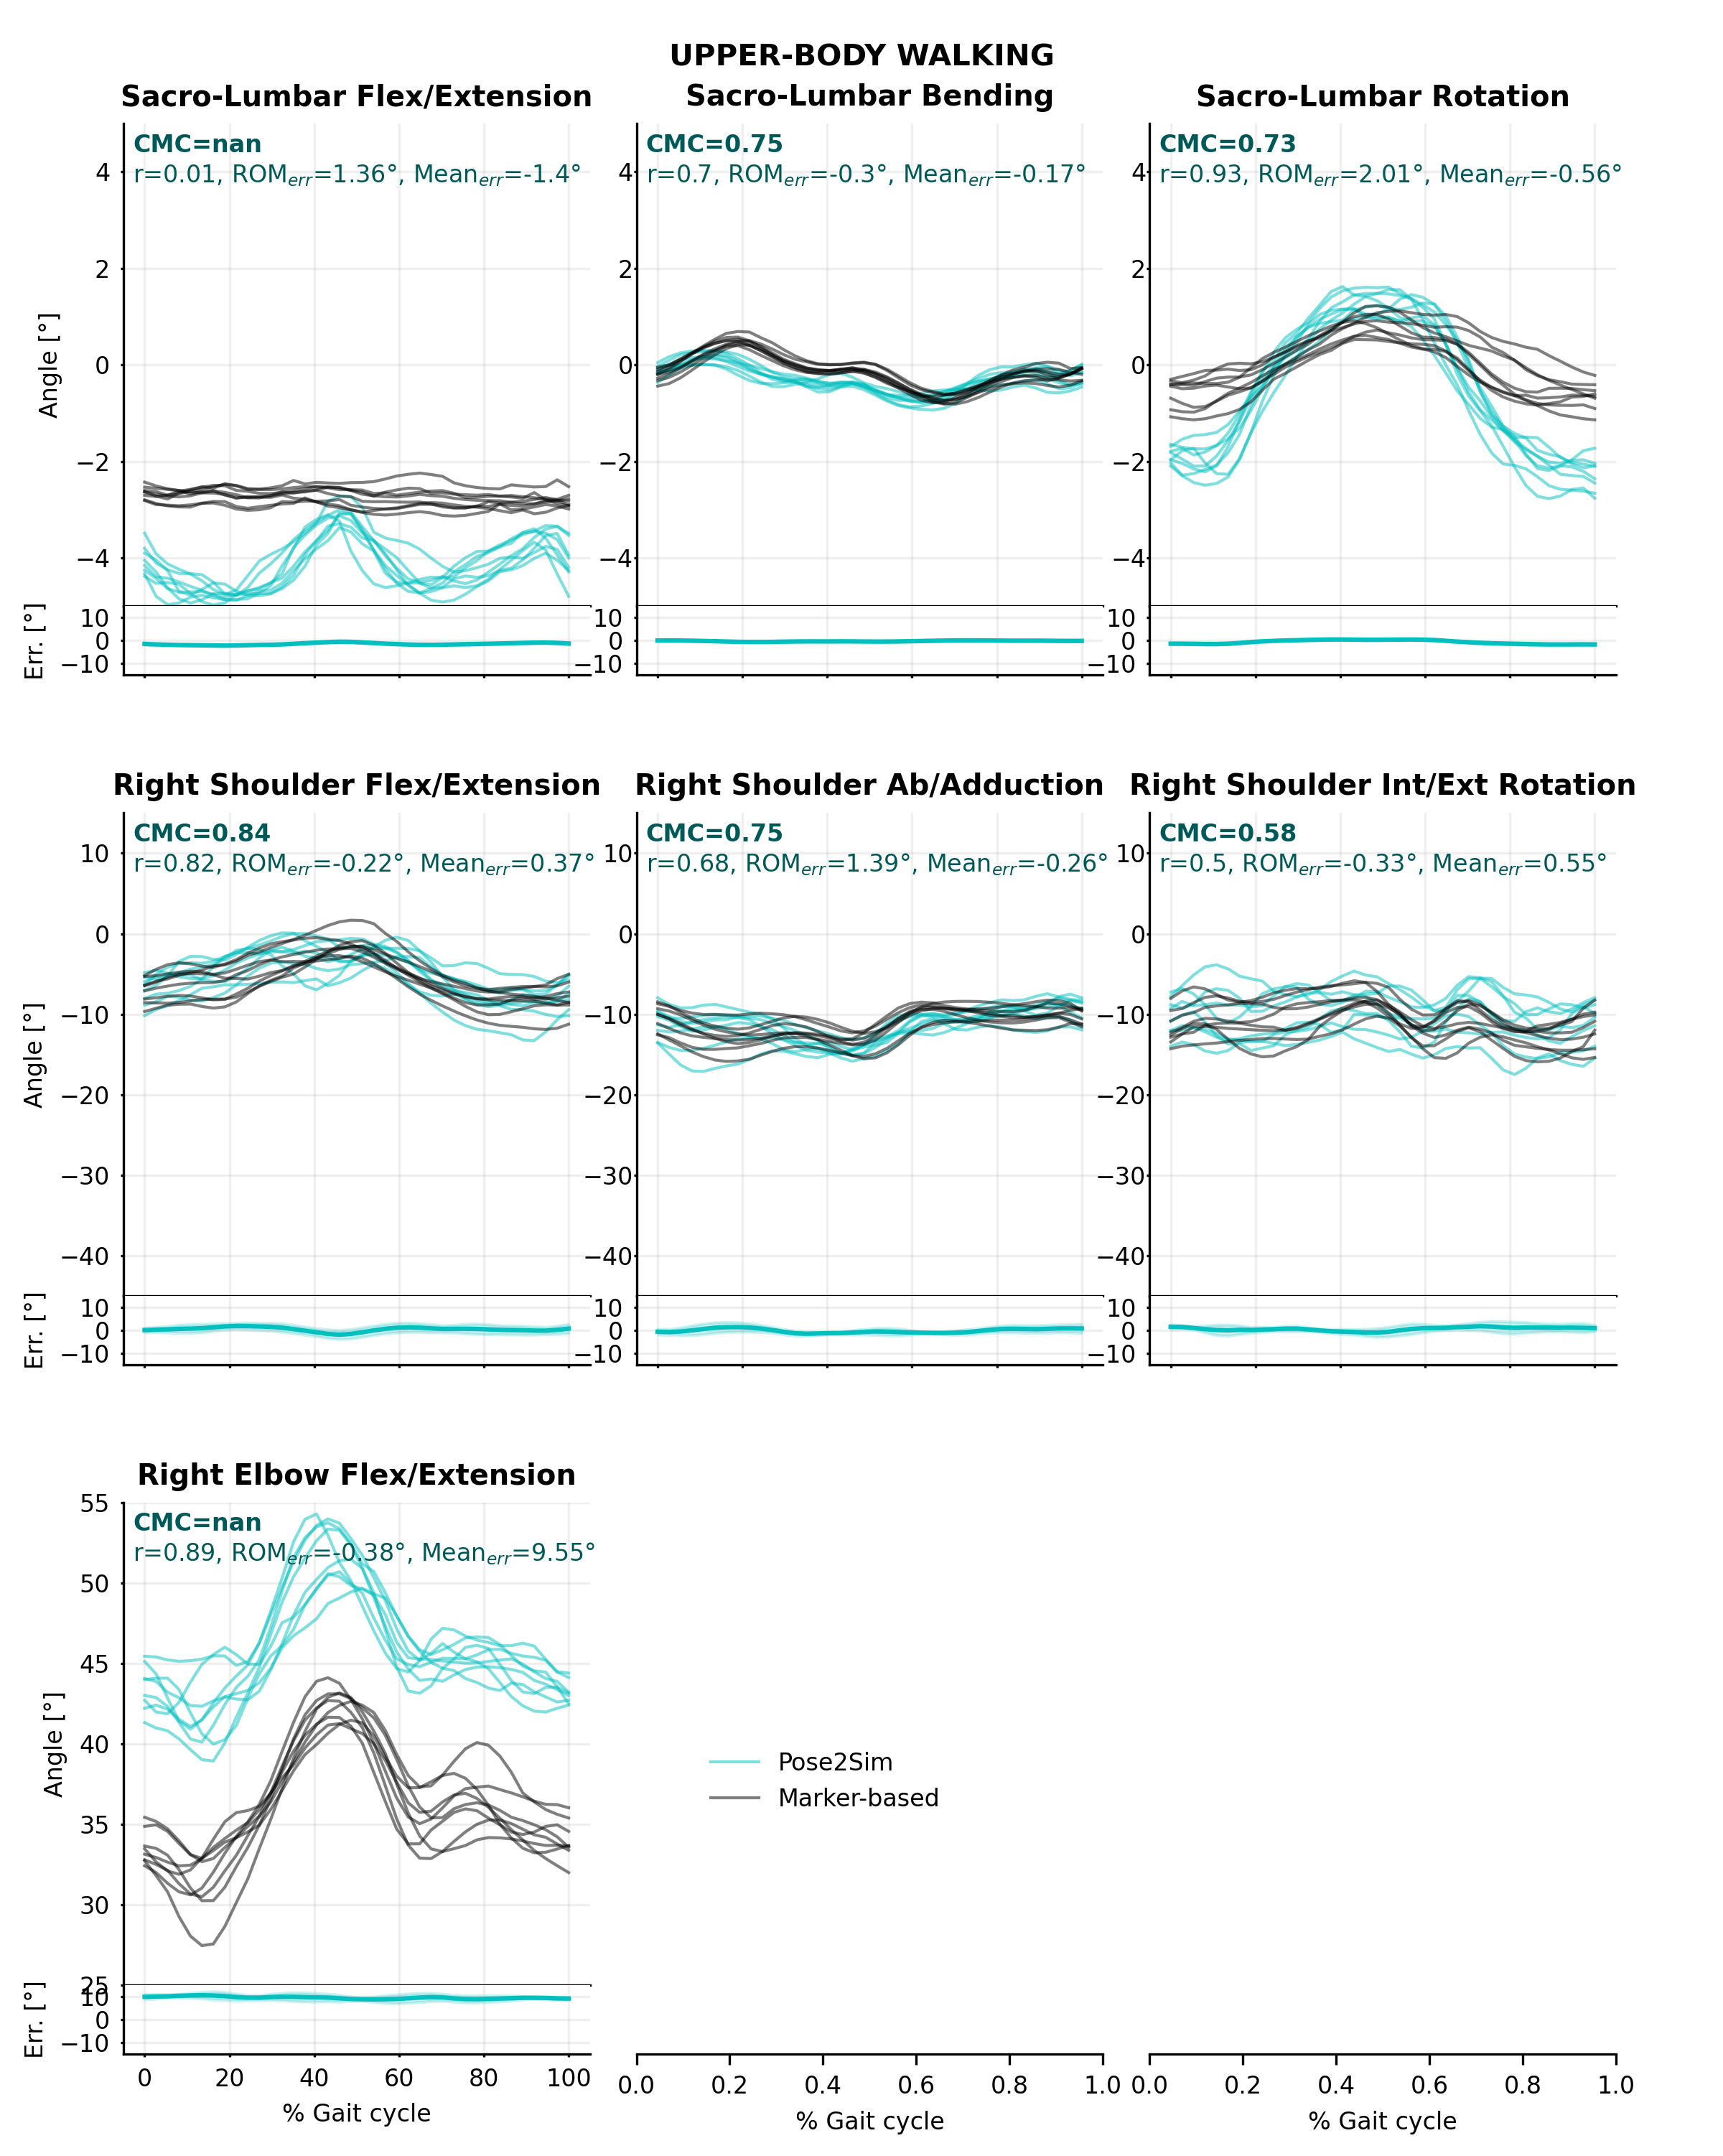
\includegraphics[height=\dimexpr\textheight-119pt]{"../Annexes/Figures/Fig_QTMWalkUp.png"}
	\caption{Pose2Sim (cyan) and marker-based (black) sacro-lumbar and upper-body joint angles for the walking task. Coefficient of multiple correlation (CMC) is indicated, and broken down into, respectively, Pearson’s coefficient (r) for correlation assessment, range of motion errors (\(ROM_{err}\)) for gain, and overall mean error (\(Mean_{err}\)) for offset. Mean error and standard deviations are also represented at the bottom of the graphics.}
	\label{fig_qtmwalkup}
\end{figure}

\begin{figure}[!ht]
	\centering
	\def\svgwidth{1\columnwidth}
	\fontsize{10pt}{10pt}\selectfont
	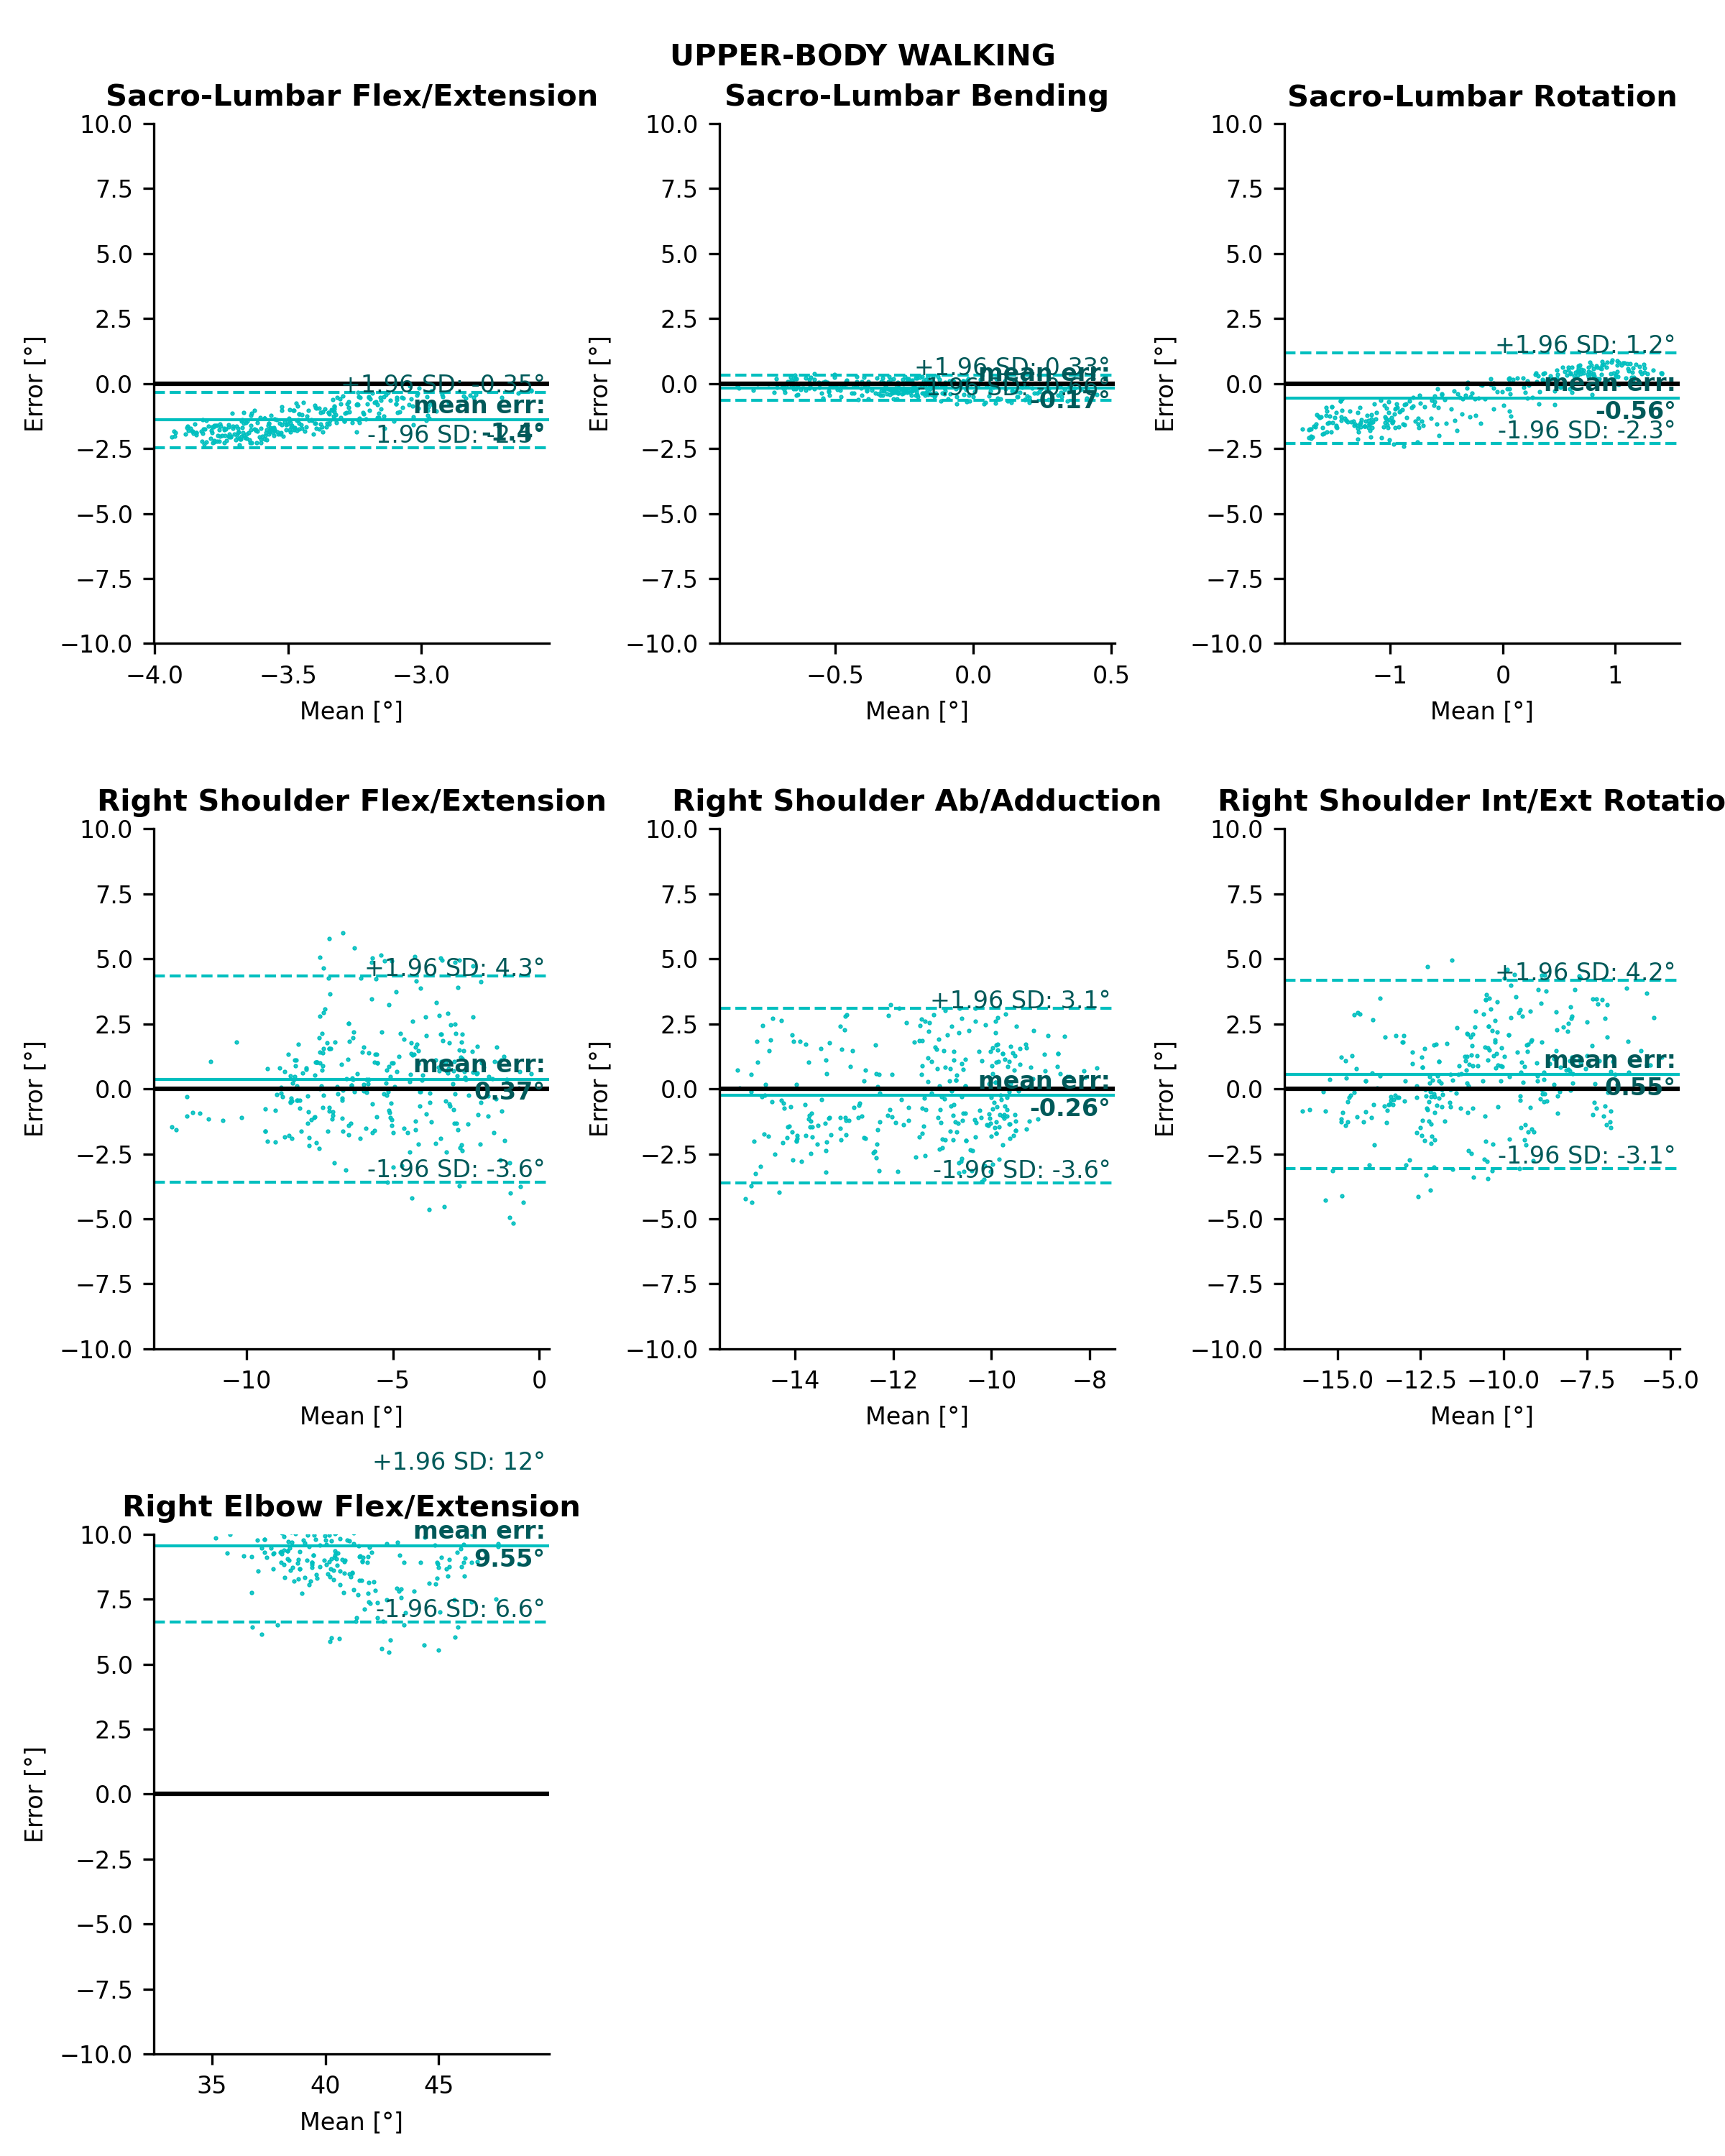
\includegraphics[height=\dimexpr\textheight-119pt]{"../Annexes/Figures/Fig_BlandWalkUp.png"}
	\caption{Bland–Altman analysis of sacro-lumbar and upper-body joint angle errors for the walking task. Mean bias is represented as a horizontal solid, bold line, and 95\% limits of agreement are represented as dotted lines.}
	\label{fig_blandwalkup}
\end{figure}

\clearpage
\subsection{Accuracy: Upper-body results for the running task}

\begin{figure}[!ht]
	\centering
	\def\svgwidth{1\columnwidth}
	\fontsize{10pt}{10pt}\selectfont
	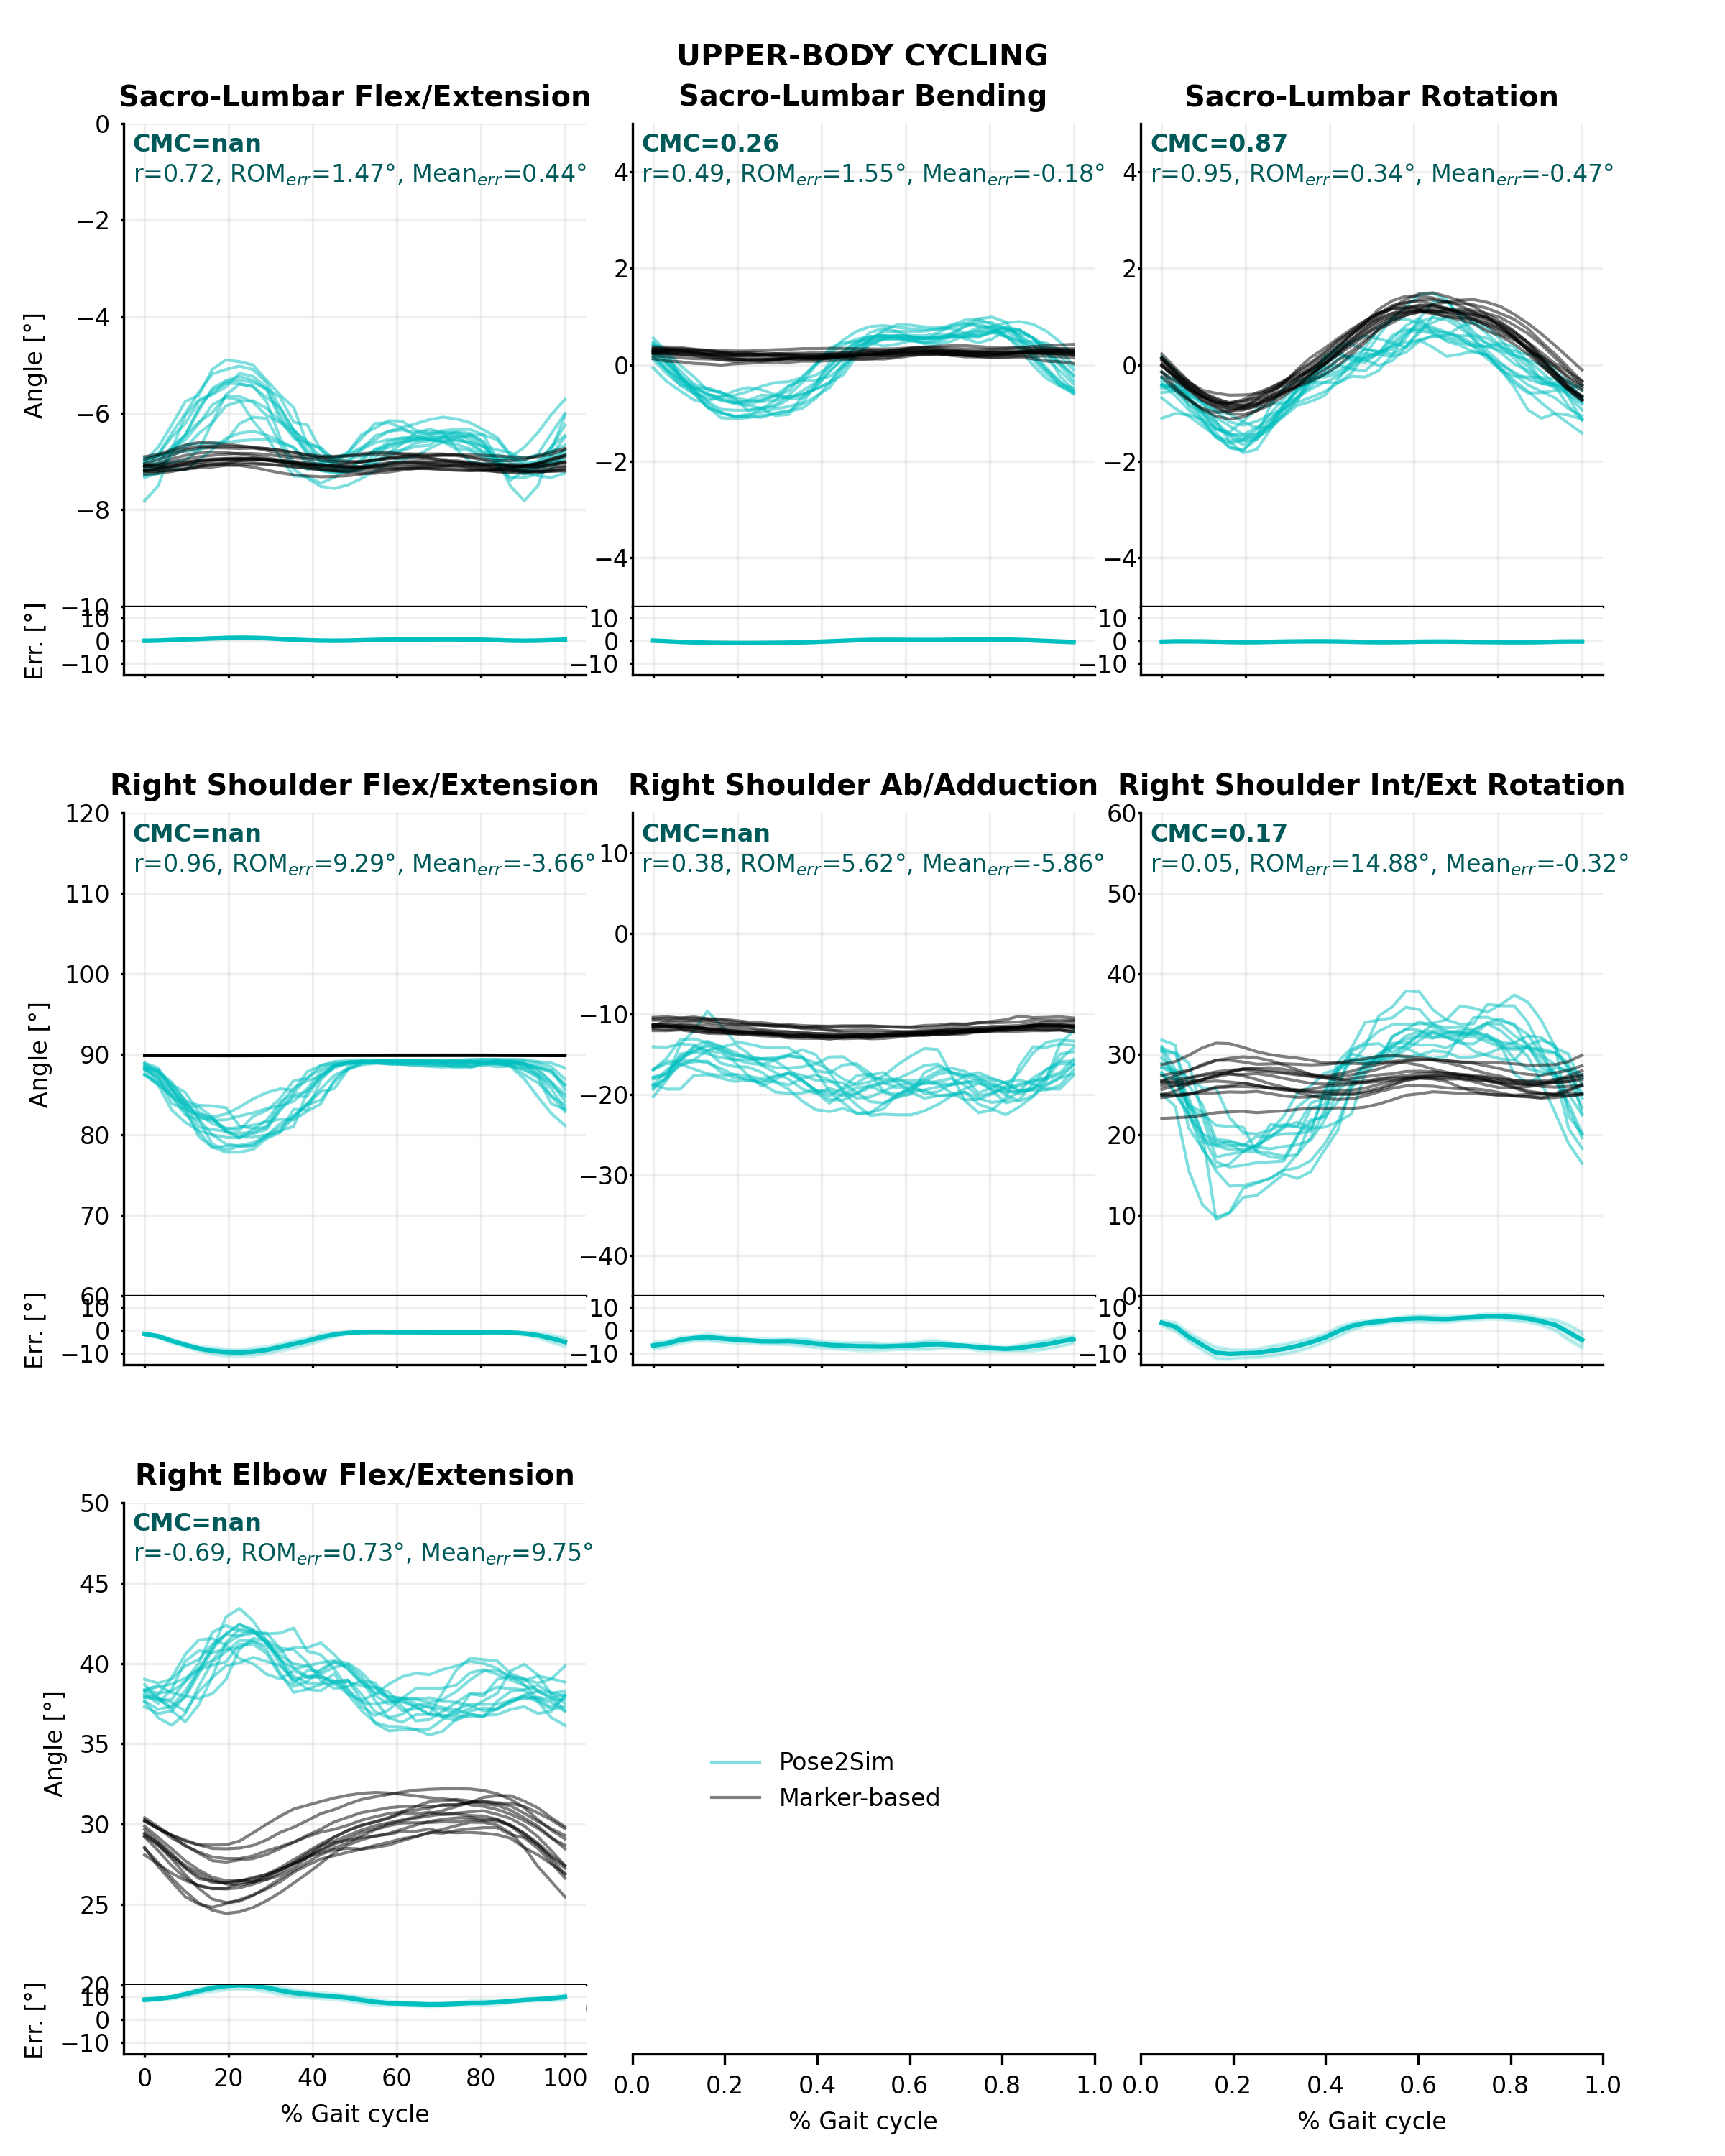
\includegraphics[height=\dimexpr\textheight-119pt]{"../Annexes/Figures/Fig_QTMBikeUp.png"}
	\caption{Pose2Sim (cyan) and marker-based (black) sacro-lumbar and upper-body joint angles for the running task. Coefficient of multiple correlation (CMC) is indicated, and broken down into, respectively, Pearson’s coefficient (r) for correlation assessment, range of motion errors (\(ROM_{err}\)) for gain, and overall mean error (\(Mean_{err}\)) for offset. Mean error and standard deviations are also represented at the bottom of the graphics.}
	\label{fig_qtmrunup}
\end{figure}

\begin{figure}[!ht]
	\centering
	\def\svgwidth{1\columnwidth}
	\fontsize{10pt}{10pt}\selectfont
	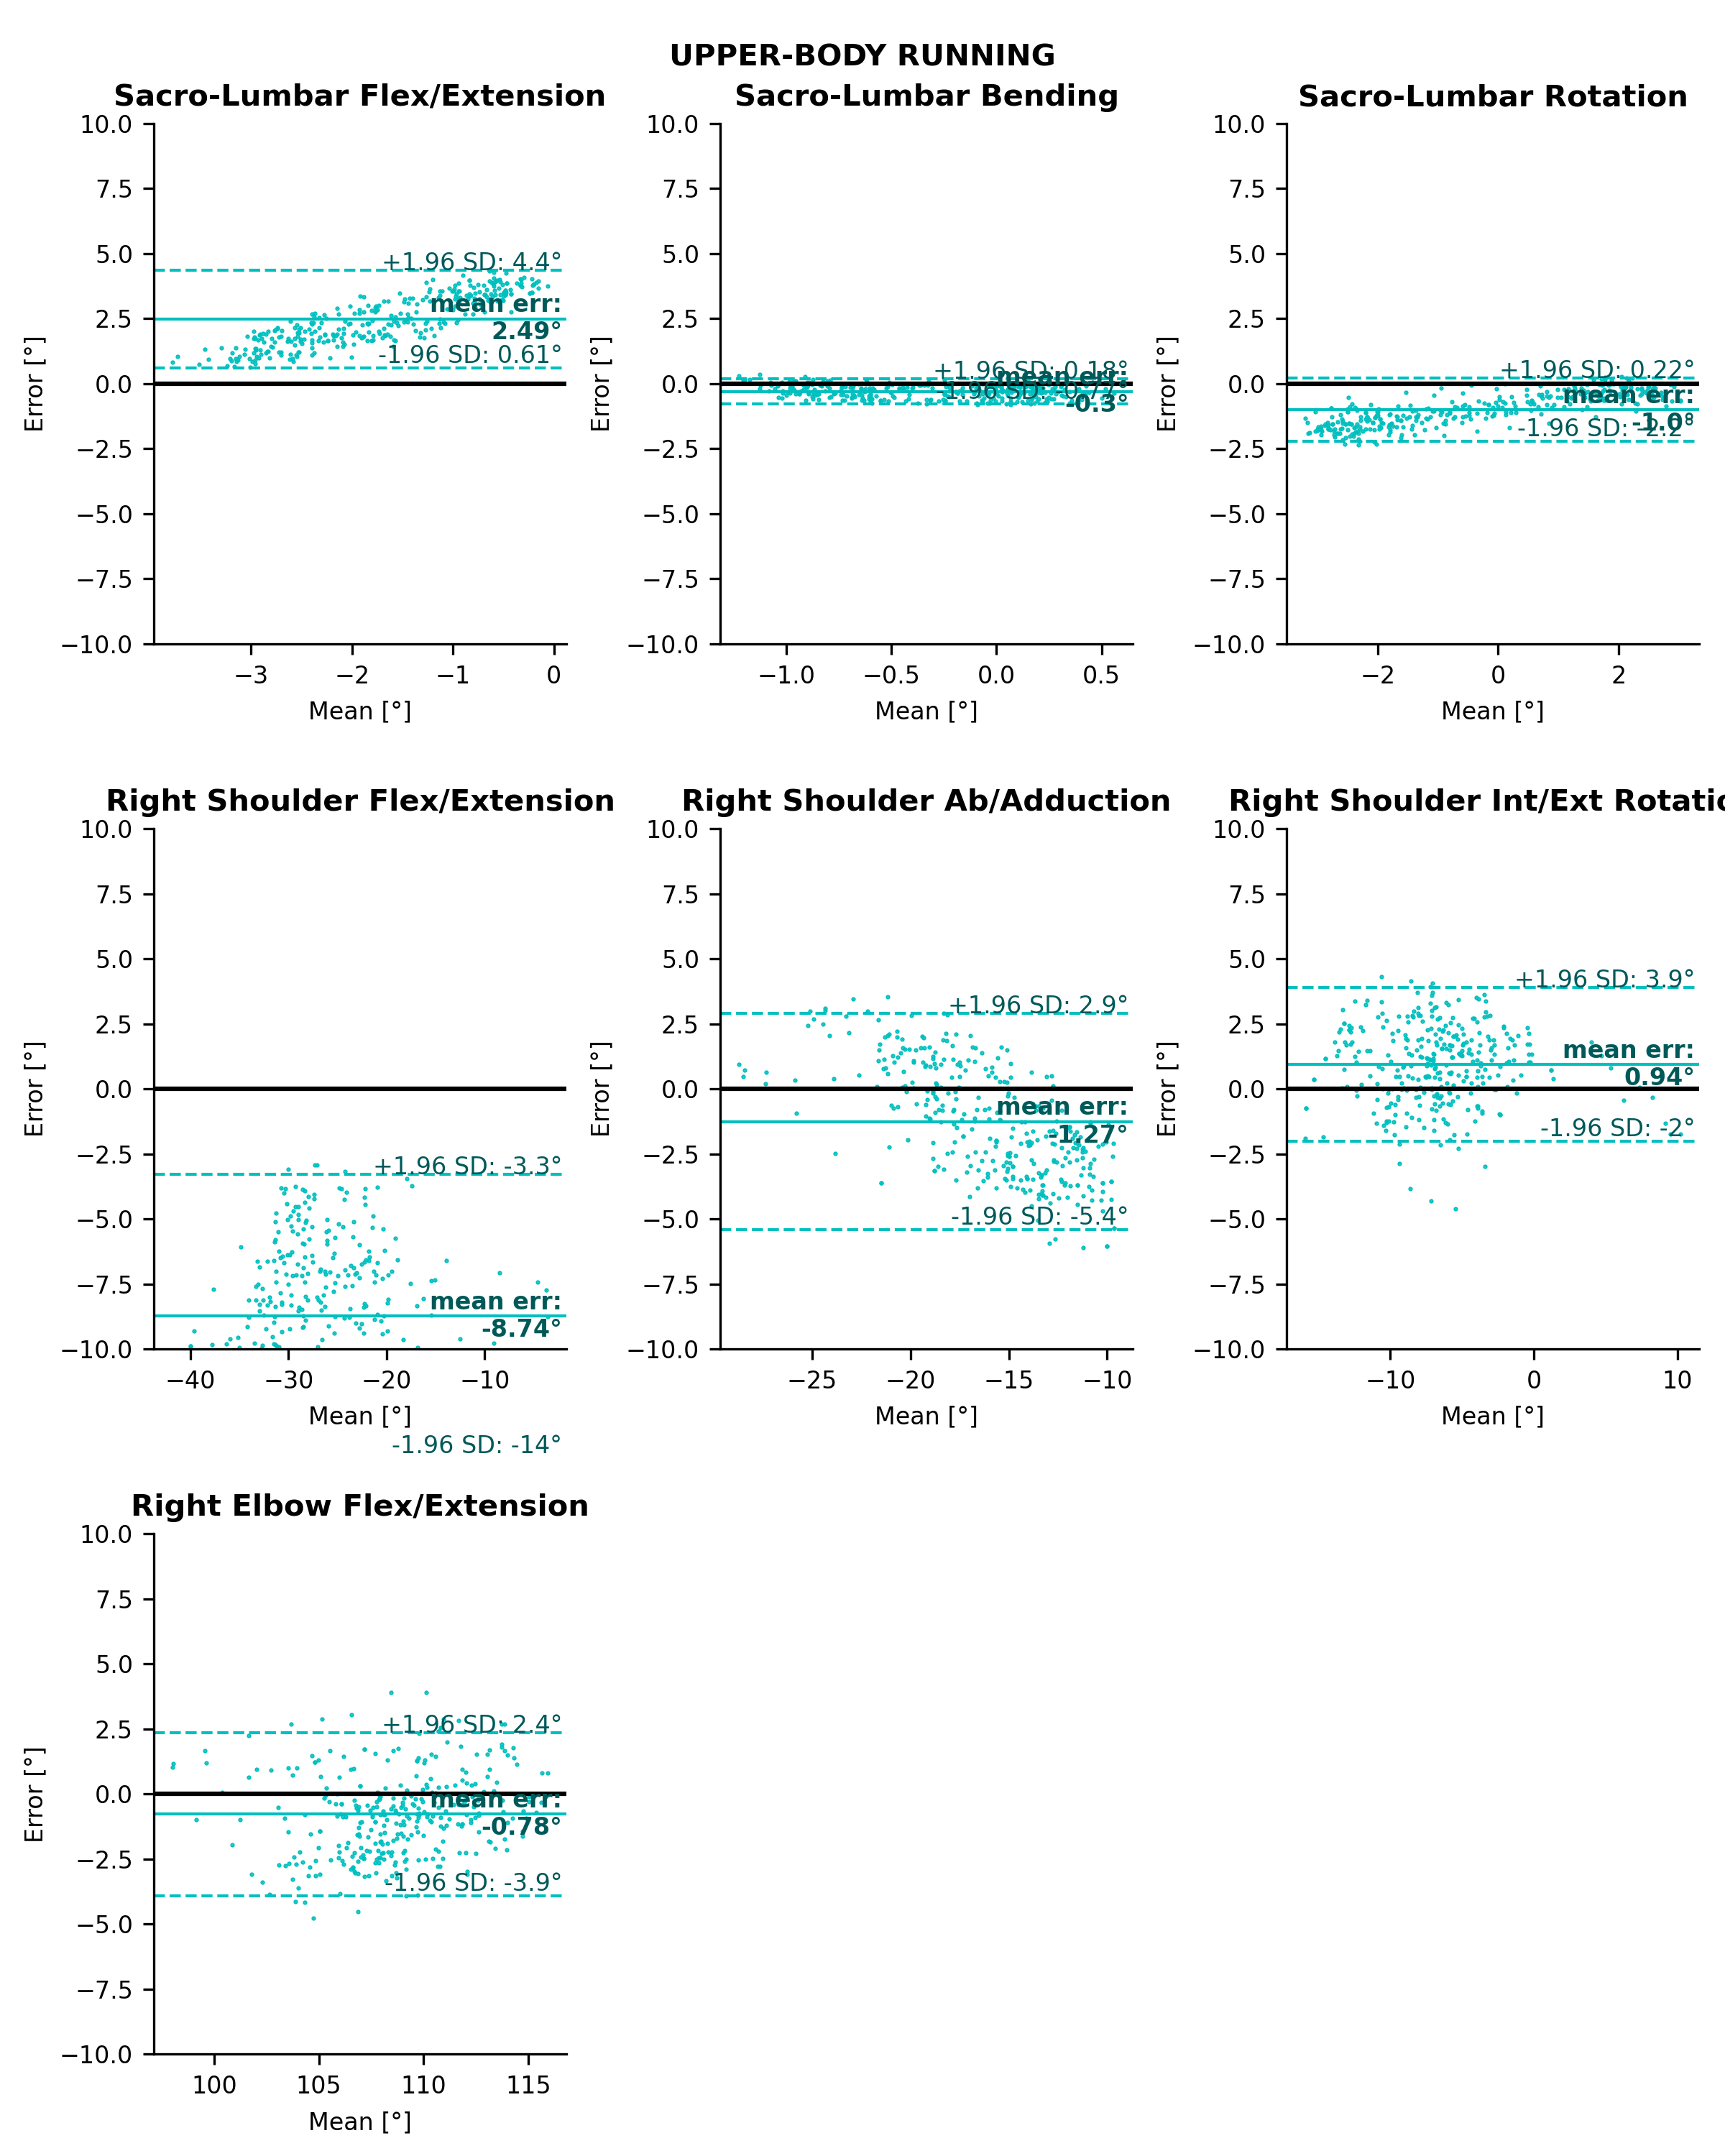
\includegraphics[height=\dimexpr\textheight-119pt]{"../Annexes/Figures/Fig_BlandRunUp.png"}
	\caption{Bland–Altman analysis of sacro-lumbar and upper-body joint angle errors for the running task. Mean bias is represented as a horizontal solid, bold line, and 95\% limits of agreement are represented as dotted lines.}
	\label{fig_blandrunup}
\end{figure}


\clearpage
\subsection{Accuracy: Upper-body results for the cycling task}

\begin{figure}[!ht]
	\centering
	\def\svgwidth{1\columnwidth}
	\fontsize{10pt}{10pt}\selectfont
	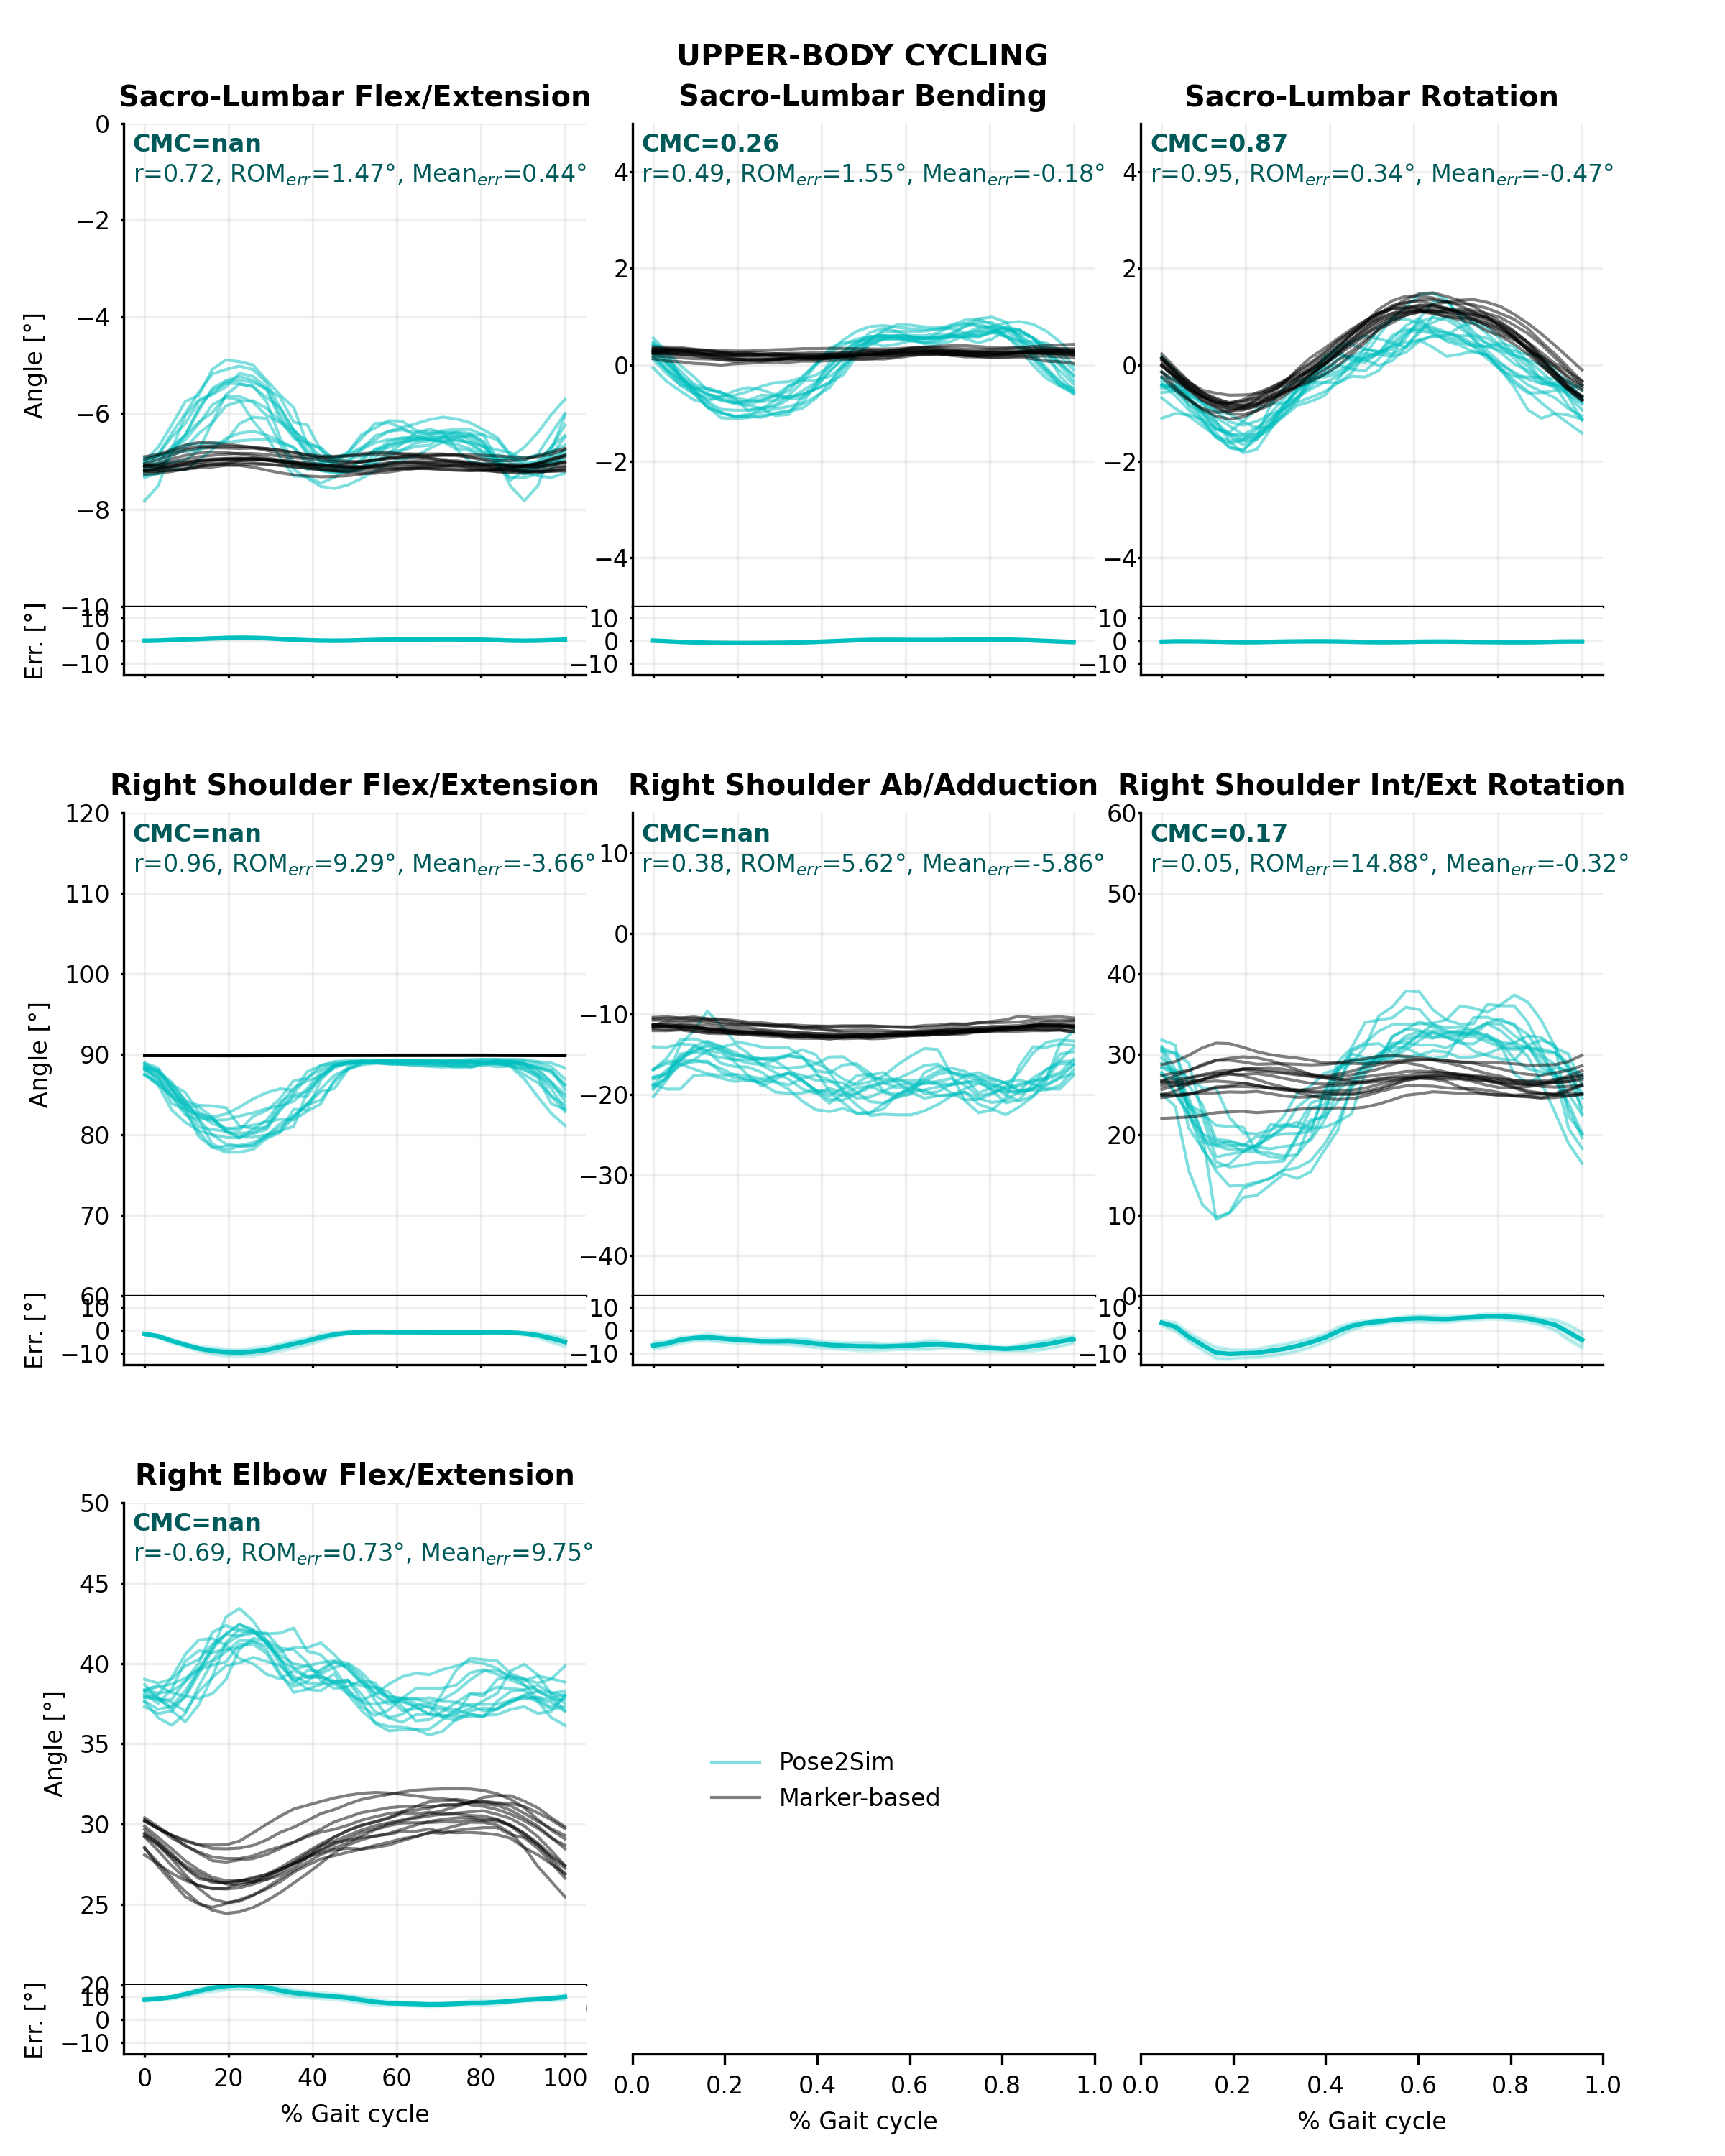
\includegraphics[height=\dimexpr\textheight-119pt]{"../Annexes/Figures/Fig_QTMBikeUp.png"}
	\caption{Pose2Sim (cyan) and marker-based (black) sacro-lumbar and upper-body joint angles for the cycling task. Coefficient of multiple correlation (CMC) is indicated, and broken down into, respectively, Pearson’s coefficient (r) for correlation assessment, range of motion errors (\(ROM_{err}\)) for gain, and overall mean errors (\(Mean_{err}\)) for offset. Mean error and standard deviations are also represented at the bottom of the graphics.}
	\label{fig_qtmbikeup}
\end{figure}

\begin{figure}[!ht]
	\centering
	\def\svgwidth{1\columnwidth}
	\fontsize{10pt}{10pt}\selectfont
	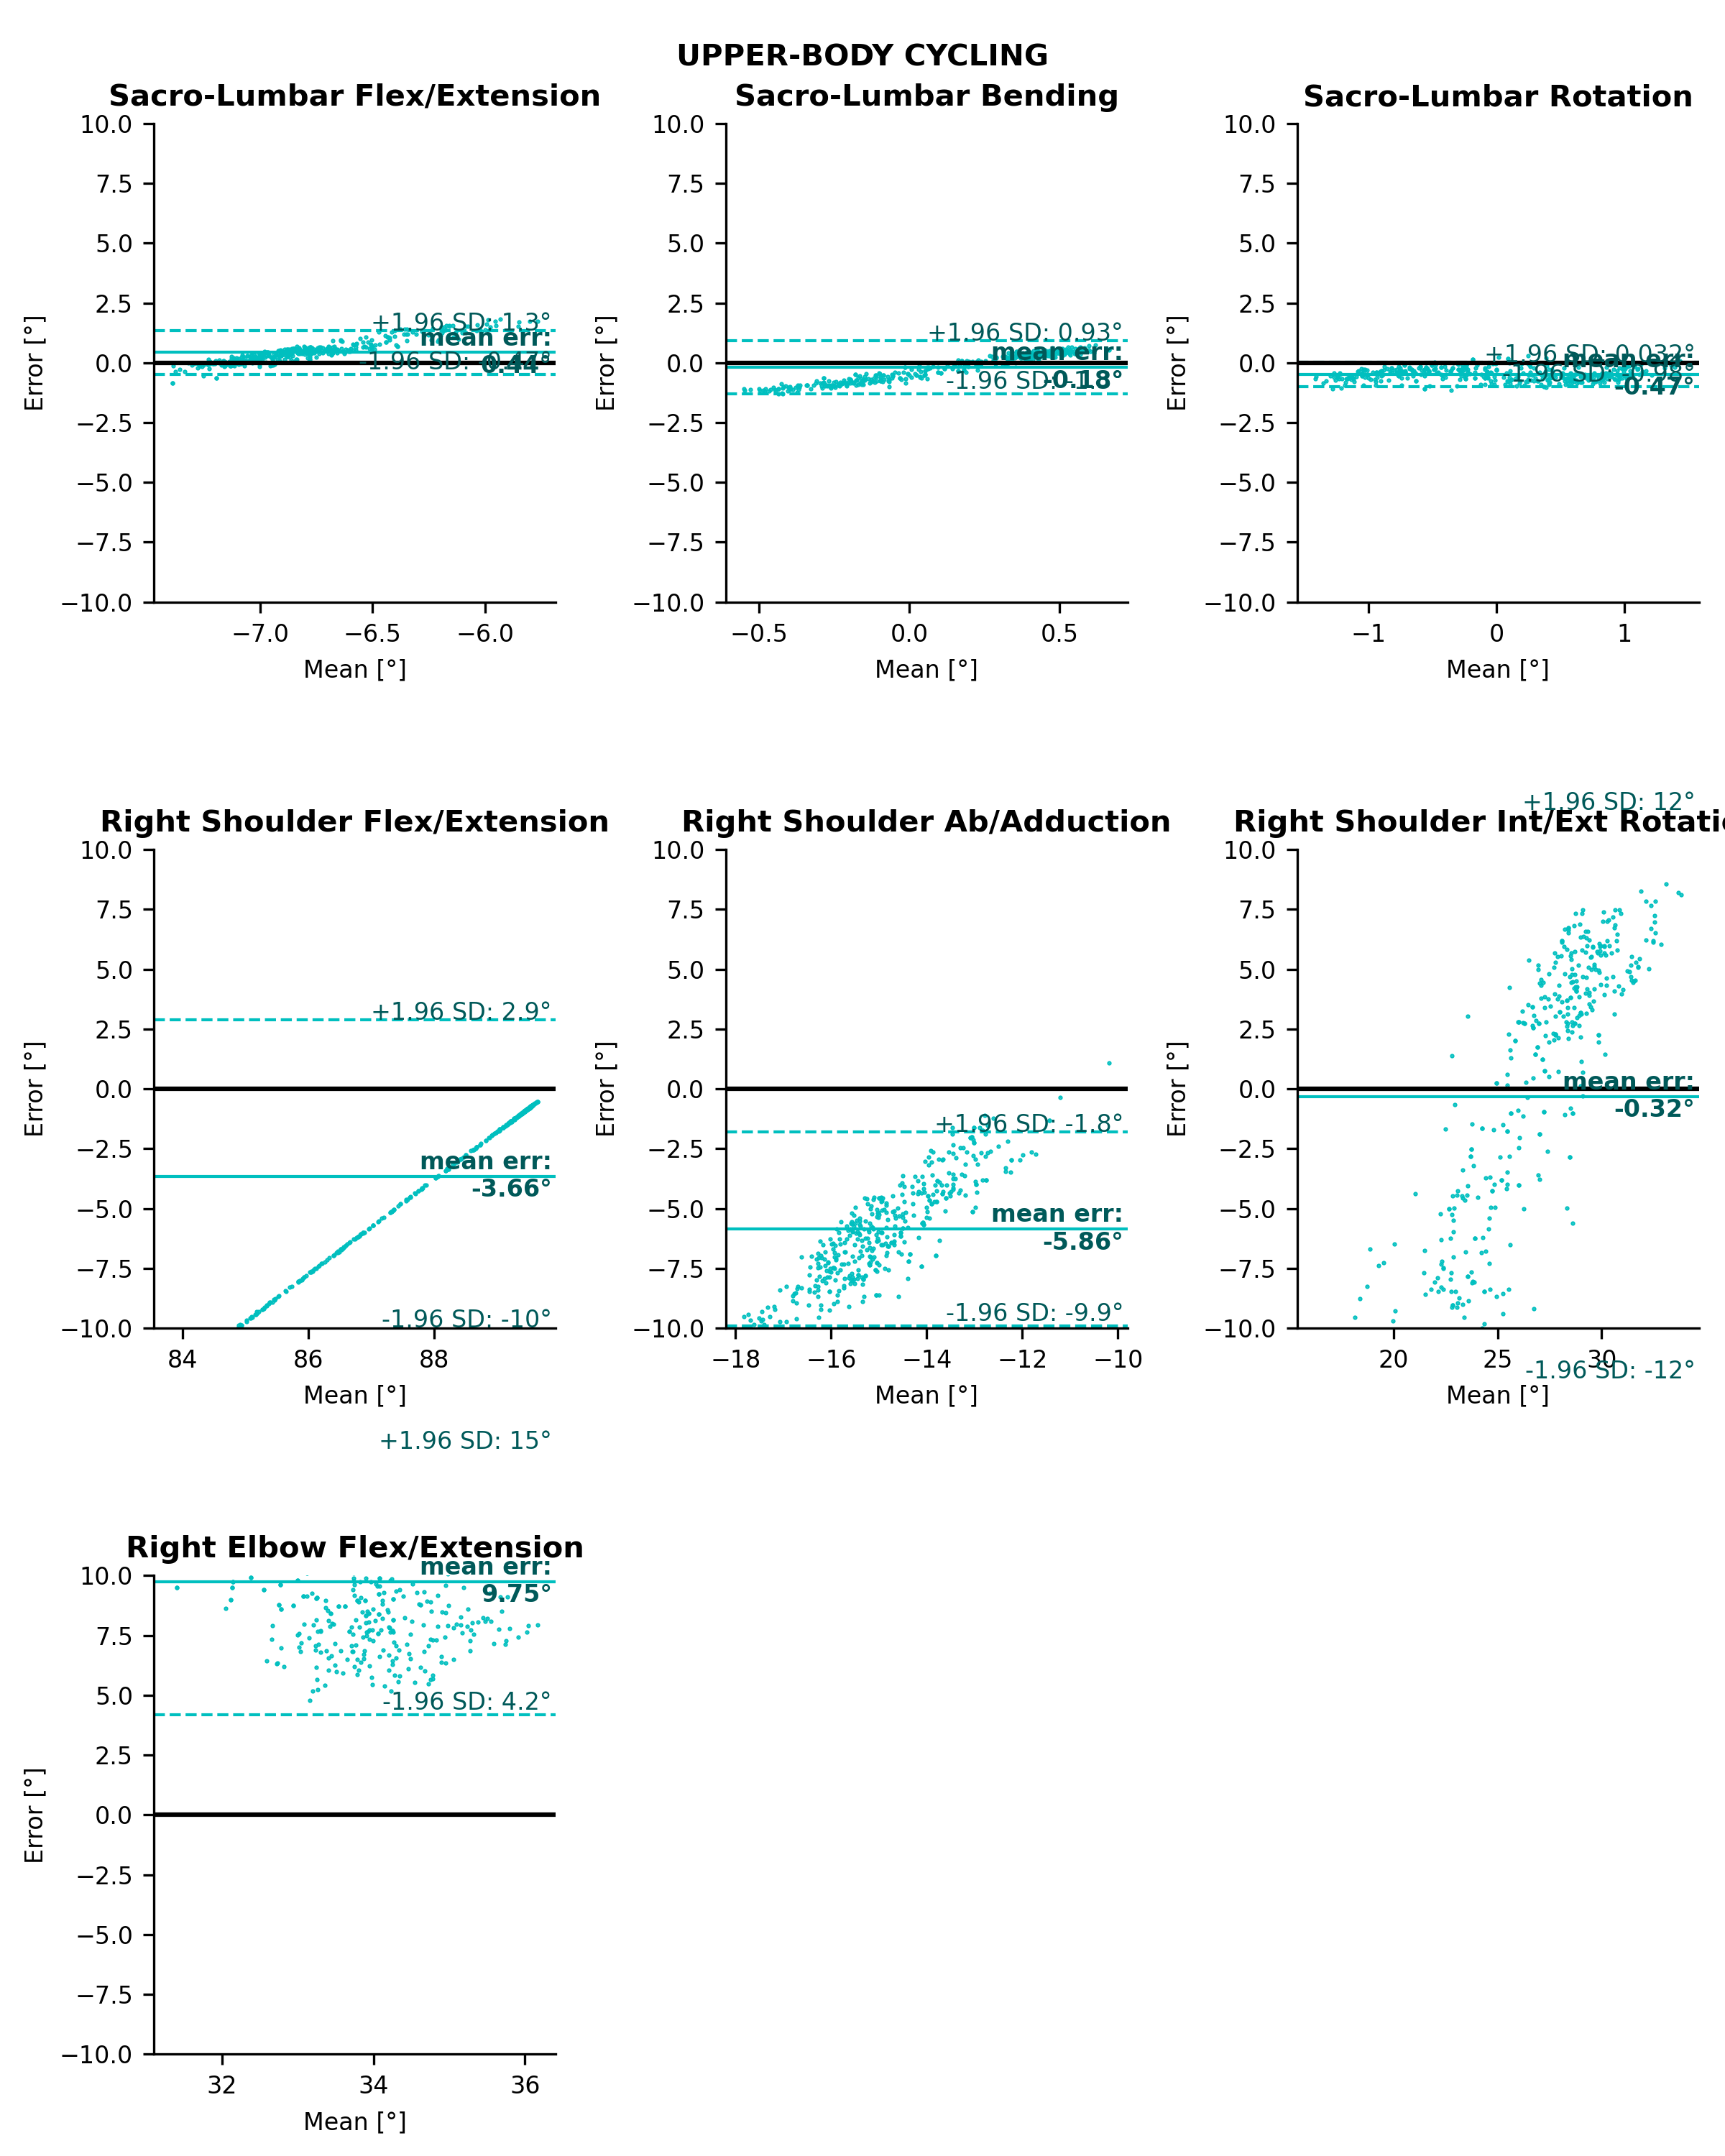
\includegraphics[height=\dimexpr\textheight-119pt]{"../Annexes/Figures/Fig_BlandBikeUp.png"}
	\caption{Bland–Altman analysis of sacro-lumbar and upper-body joint angle errors for the cycling task. Mean bias is represented as a horizontal solid, bold line, and 95\% limits of agreement are represented as dotted lines.}
	\label{fig_blandbikeup}
\end{figure}


\FloatBarrier
\chapter{Appendix C : Protocol}
\label{Ann:3}

%==============================================================================	Résumé du chapitre

\begin{center}
\rule{0.7\linewidth}{.5pt}
\begin{minipage}{0.7\linewidth}
\smallskip

\textit{Summary here on protocol.
}

%\smallskip
\end{minipage}
\smallskip
\rule{0.7\linewidth}{.5pt}
\end{center}

\minitoc
\newpage



Protocol



\section{Section 1}
\subsection{Sous section 1}
\blindtext
\subsection{Sous section 2}
\blindtext



